\documentclass[aspectratio=169]{beamer}

\usepackage[utf8]{inputenc}

\usepackage{amsfonts}
\usepackage{amsmath}
\usepackage{color}
\usepackage{listings}
\usepackage{tikz}
\usepackage{hyperref}
\usepackage[normalem]{ulem}

\newif\ifnotes
  \notesfalse
%  \notestrue

\newif\iftransitions
 \transitionstrue
% \transitionsfalse

\newif\iffast
% \fasttrue
  \fastfalse

\ifnotes
\usepackage{pgfpages}
\setbeameroption{show notes}
\setbeameroption{show notes on second screen=right}
\fi

\usetheme{Rochester}
\usecolortheme{beaver}

\addtobeamertemplate{navigation symbols}{}{%
    \usebeamerfont{footline}%
    \usebeamercolor[fg]{footline}%
    \hspace{1em}%
    \insertframenumber/\inserttotalframenumber
}

\lstloadlanguages{C++}
    \lstset{%
        language={C++},
        basicstyle=\ttfamily,
        keywordstyle=\color{blue},
        showstringspaces=false,
        escapechar={§},
        escapeinside={(*@}{@*)}
    }

\lstdefinestyle{cpp20}{language={C++},
  morekeywords={noexcept,co_await,co_return,co_yield,requires,consteval,constinit,concept}
}

\tikzstyle{every picture}+=[remember picture]

\newcommand{\cpause}{\iftransitions \pause \fi}

\newcommand{\cuncover}[2]{\iftransitions \uncover<#1>{#2} \else #2 \fi}

\definecolor{co_return_object}{RGB}{179,179,255}
\definecolor{co_promise}{RGB}{255,179,179}
\definecolor{co_awaitable}{RGB}{179,255,179}


\title{Amortized $\mathcal{O}(1)$ Complexity}
\author{Andreas Weis}
\institute{}

\date{CppCon 2024}
\titlegraphic{
\includegraphics[height=.15\textheight]{resources/cppcon.png}}

\iffalse
\fi

\begin{document}
\frame{\titlepage
 \note{ This is amortized constant complexity.}
}

\iftrue %crop

\begin{frame}
  \frametitle{Runtime Complexity}
  
  \begin{center}
  \begin{itemize}
    \item $f \in \mathcal{O}(g) \iff \exists\ C > 0.\ \exists\ x_0 > 0.\ \forall\ x > x_0: |f(x)| \le C\cdot|g(x)|$
  \end{itemize}
  \end{center}

  \note{ We all know about runtime, complexity. }
\end{frame}

\begin{frame}

  \begin{center}
  \huge{Child's play!}
  \end{center}
  
  \note{ That's easy, right? }
\end{frame}

\begin{frame}
  \frametitle{What is amortized complexity?}

  \begin{center}
  \only<2-3>{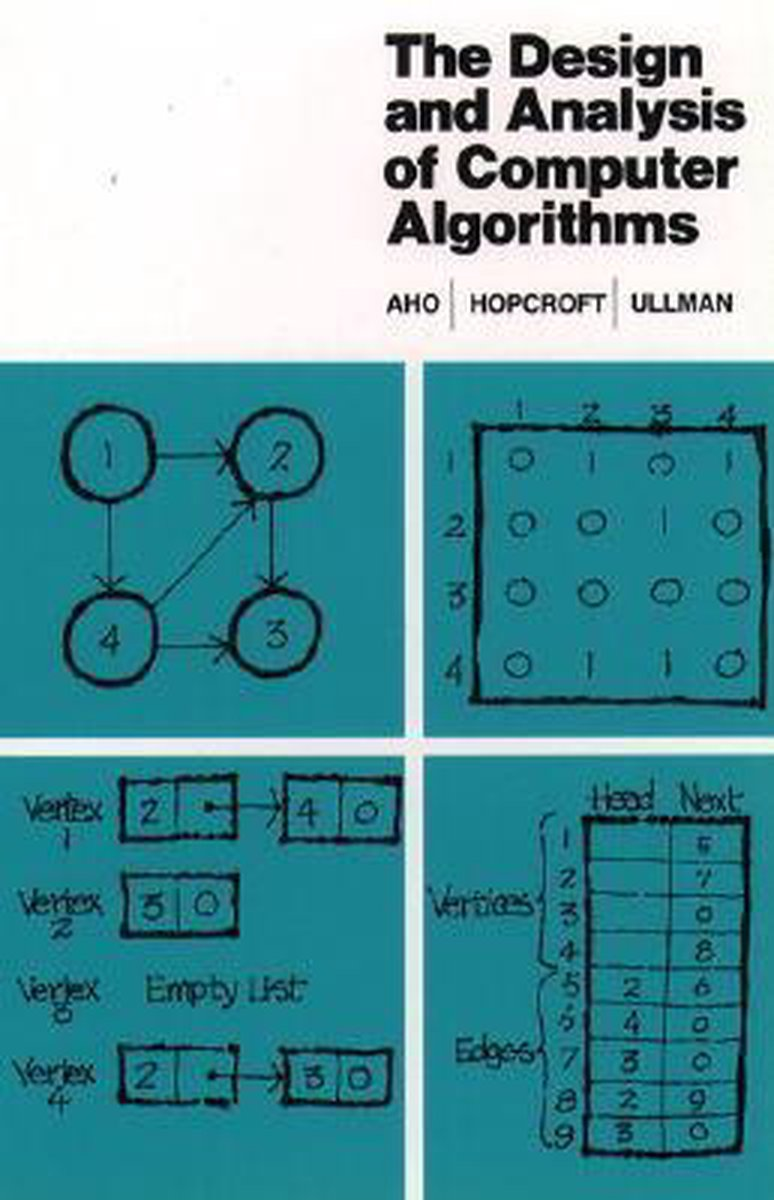
\includegraphics[height=.9\textheight]{amortizedgfx/ahu.jpg}}
  \only<4-5>{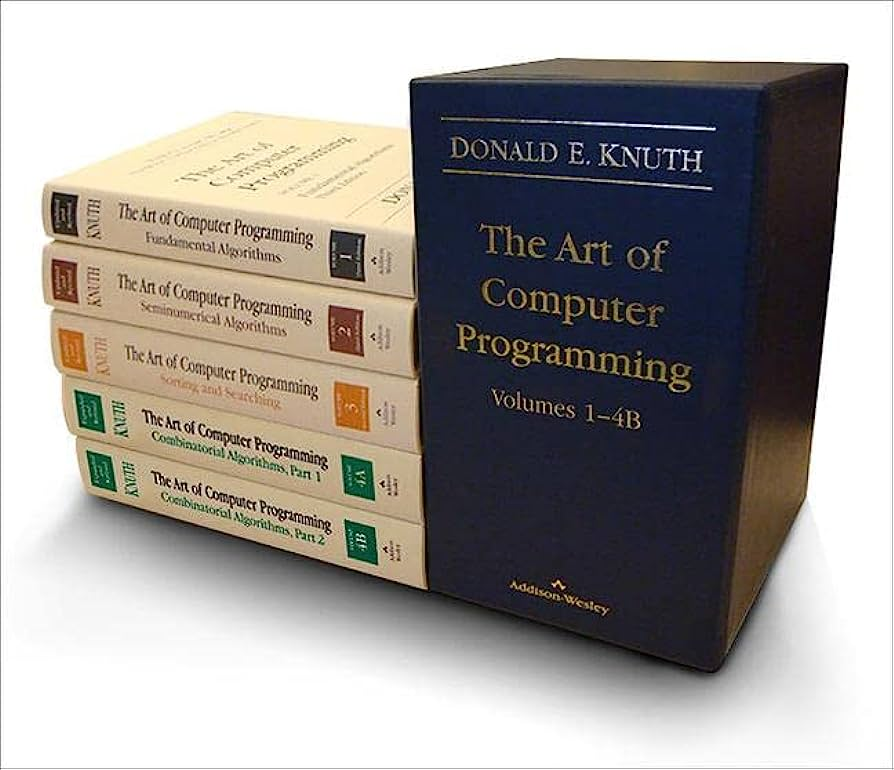
\includegraphics[height=.9\textheight]{amortizedgfx/taocp.jpg}}
  \only<6>{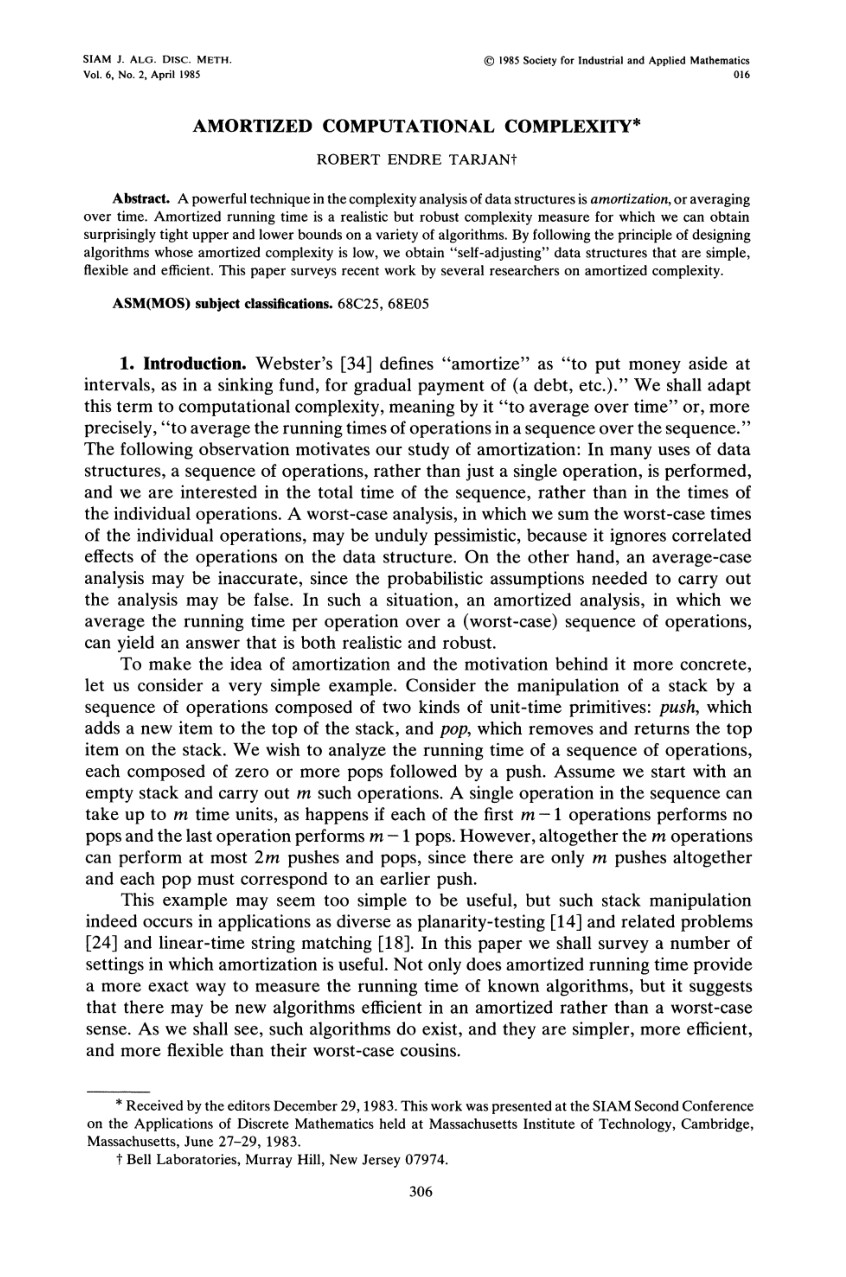
\includegraphics[height=.9\textheight]{amortizedgfx/tarjan.jpg}}
  \only<7>{
   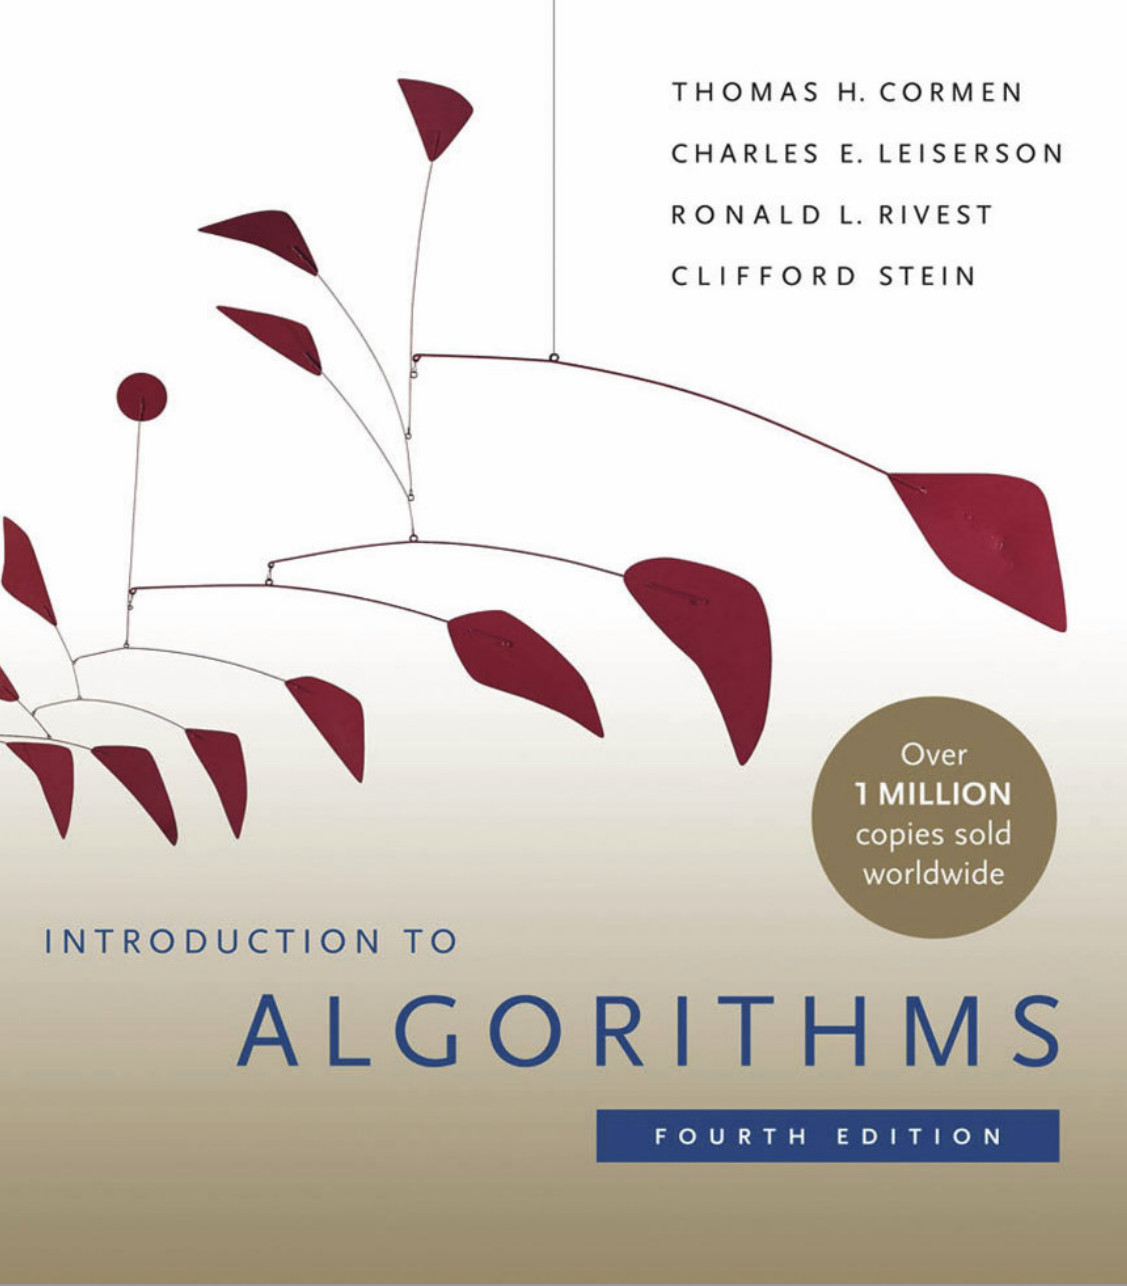
\includegraphics[height=.9\textheight]{amortizedgfx/cormen.jpg}
  }
  \end{center}
  
  \only<3,5>{
  \begin{tikzpicture}[remember picture,overlay]
  \draw[line width=30pt,red] ([shift={(0,-5em)}]current page.135) -- (current page.315);
  \draw[line width=30pt,red] ([shift={(5em,0)}]current page.215) -- ([shift={(0,-5em)}]current page.45);
  \end{tikzpicture}
  }
  
  \note{
  \begin{itemize}
  \item But what is amortized complexity?
  \item Let's check the literature.
  \item Well, there's nothing in AHU.
  \item There's nothing
  \item in Knuth.
  \item There's this paper by Tarjan, but it's kinda hard to read.
  \item Fortunately, Cormen has a whole chapter on amortized analysis, so we'll go with that.
  \end{itemize}
  }
  
\end{frame}

\begin{frame}

  \frametitle{Amortized Analysis}
  
  \begin{itemize}
    \item Aggregate analysis
    \alert<2>{\item Accounting method}
    \item Potential method
  \end{itemize}
  
  \note{
  \begin{itemize}
  \item They discuss three different methods.
  \item And we will look at accounting, because that is by far the coolest of the three.
  \end{itemize}
  }
\end{frame}

\begin{frame}
  \frametitle{Accounting}
  
  \begin{center}
  \only<1>{ 
\includegraphics[height=.9\textheight]{amortizedgfx/question_block.png} }
  \only<2>{ 
\includegraphics[height=.9\textheight]{amortizedgfx/coin.png} }
  \end{center}
  
  \note{
  \begin{itemize}
    \item So what is accounting all about?
    \item Coins! It's about coins! We use coins to pay for computational steps and the number of coins required is a measure for the complexity.
  \end{itemize}
  }
\end{frame}

\begin{frame}[fragile]
  \frametitle{Setting up a \texttt{vector}}
  
  \begin{lstlisting}[style=cpp20]
  std::vector<int> v(2, 0);
  v.reserve(4);
  \end{lstlisting}
  
  \pause
  
  \begin{center}
  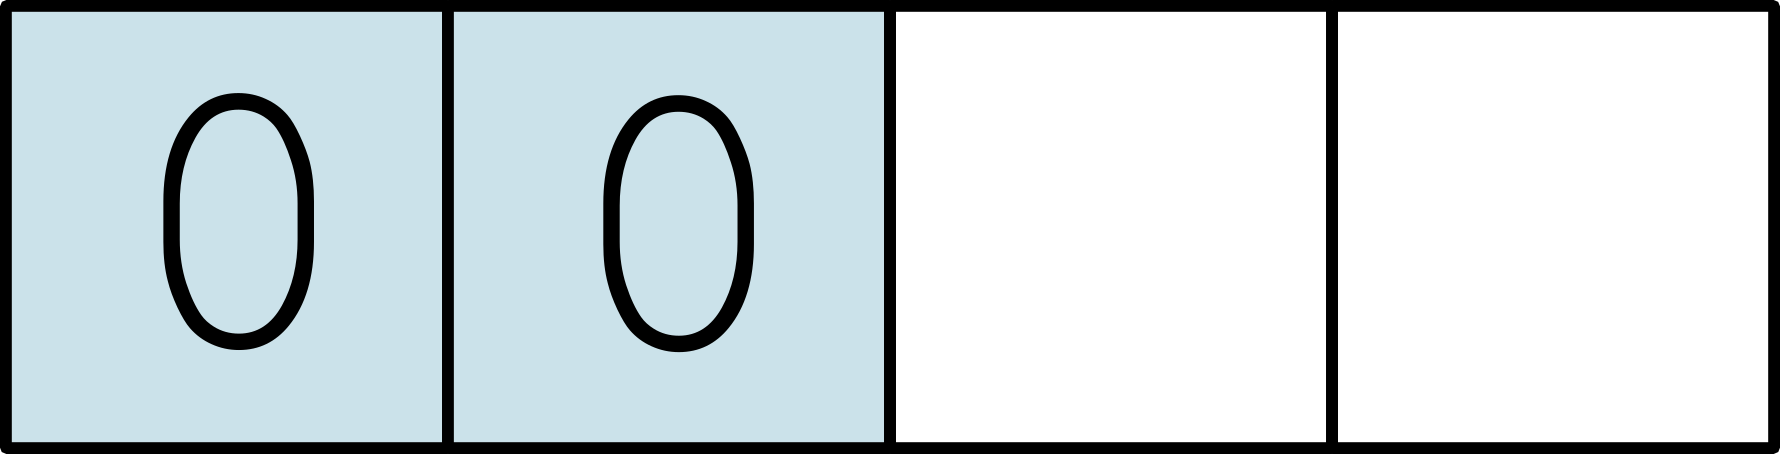
\includegraphics[width=.5\textwidth]{amortizedgfx/push_000.png}
  \end{center}
  
  \note{
  \begin{itemize}
    \item So let's set up a little vector.
    \item And now let's push some elements into it.
  \end{itemize}
  }
\end{frame}

\begin{frame}[fragile]
  \frametitle{Cost of \texttt{vector::push\_back}}
  
  
\includegraphics[width=.1\textwidth]{amortizedgfx/coin_01.png}
  
  \begin{lstlisting}[style=cpp20]
  v.push_back(1);
  \end{lstlisting}
  
  \begin{center}
  
\includegraphics[width=.5\textwidth]{amortizedgfx/push_001.png}
  \end{center}
  
  \note{
  When we push the first element, we have to spend one coin for copying the element.
  }
\end{frame}

\begin{frame}[fragile]
  \frametitle{Cost of \texttt{vector::push\_back}}
  
  
\includegraphics[width=.1\textwidth]{amortizedgfx/coin_01.png}
  
  \begin{lstlisting}[style=cpp20]
  v.push_back(2);
  \end{lstlisting}
  
  \begin{center}
  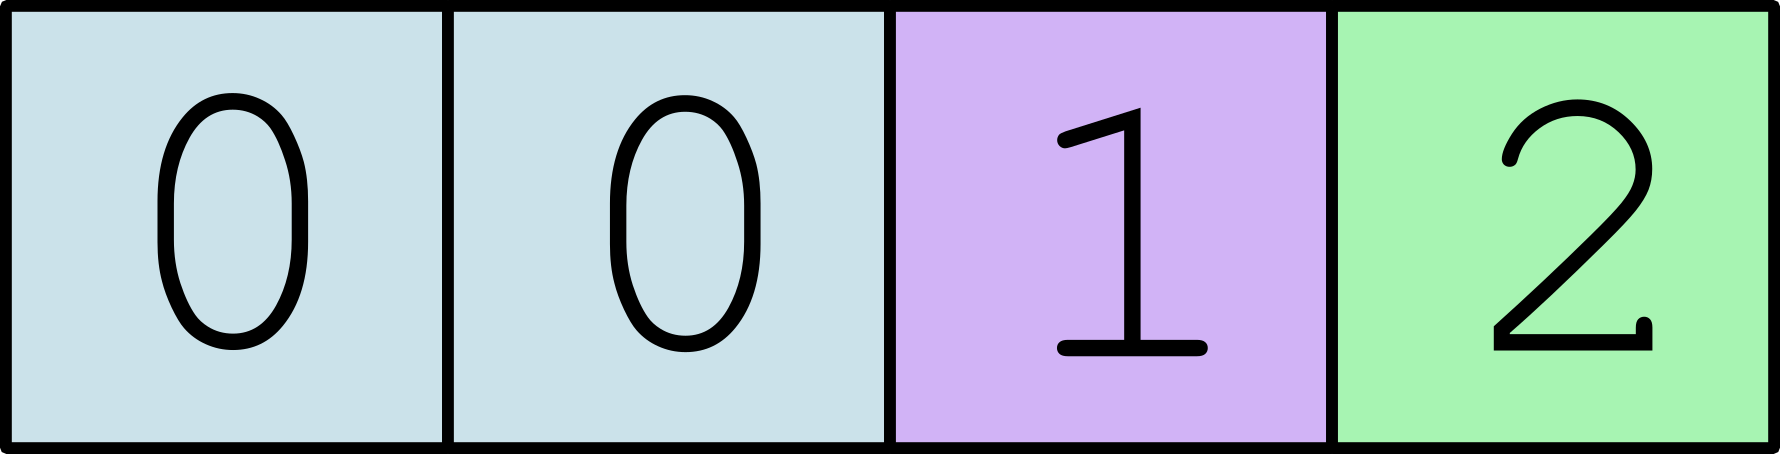
\includegraphics[width=.5\textwidth]{amortizedgfx/push_002.png}
  \end{center}
  
  \note{
  We push a second element and again we have to spend one coin for the copy.
  }
\end{frame}

\begin{frame}[fragile]
  \frametitle{Cost of \texttt{vector::push\_back}}

  \only<2>{ \vspace{.25\textheight} }
  \only<3>{ 
\includegraphics[height=.25\textheight]{amortizedgfx/coin_01.png} }
  \only<4>{ 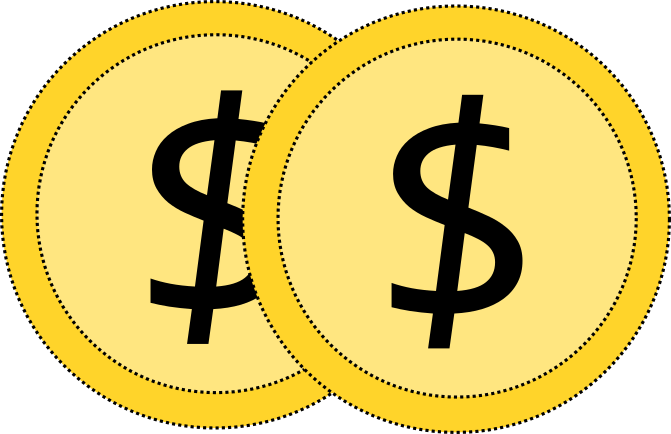
\includegraphics[height=.25\textheight]{amortizedgfx/coin_02.png} }
  \only<5>{ 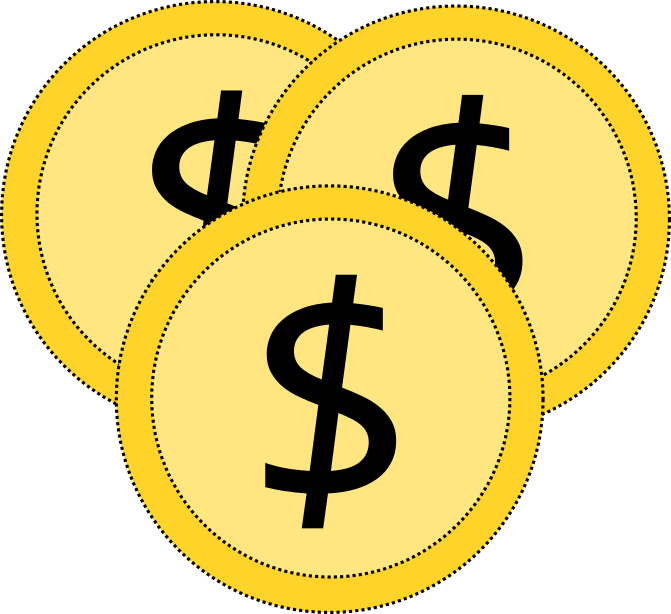
\includegraphics[height=.25\textheight]{amortizedgfx/coin_03.png} }
  \only<6>{ 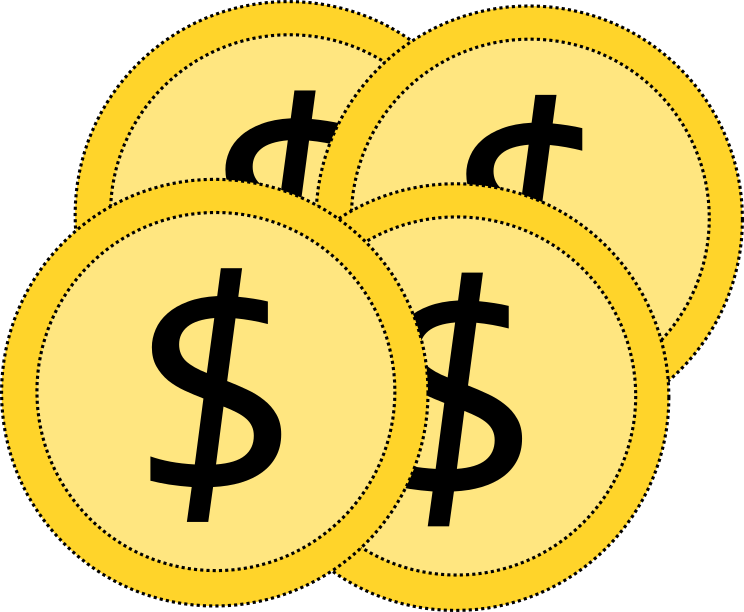
\includegraphics[height=.25\textheight]{amortizedgfx/coin_04.png} }
  \only<7>{ 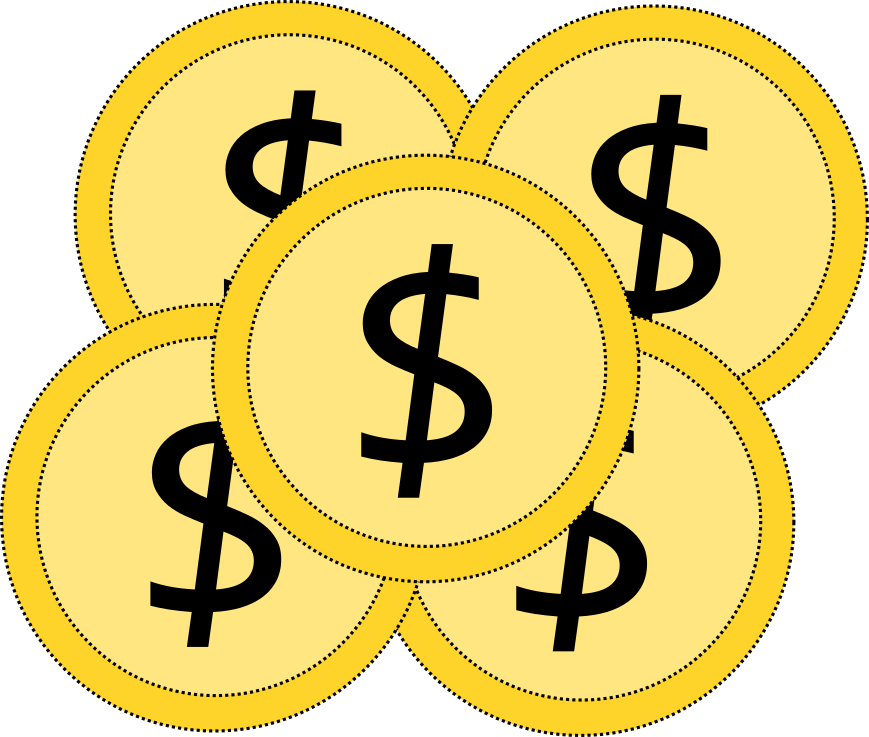
\includegraphics[height=.25\textheight]{amortizedgfx/coin_05.png} }

  \begin{lstlisting}[style=cpp20]
  v.push_back(3);
  \end{lstlisting}
  
  \only<1>{\begin{center} 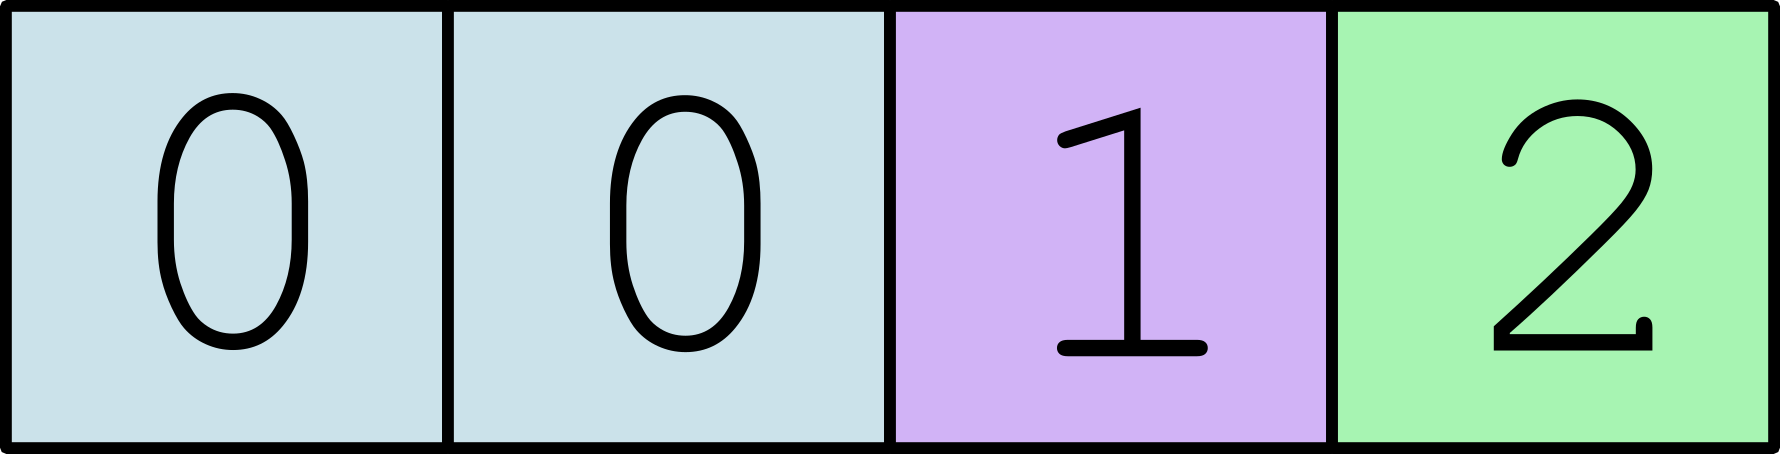
\includegraphics[width=.5\textwidth]{amortizedgfx/push_002.png} \end{center} \vspace{10pt} No room! }
  \only<2>{
  \begin{center}
  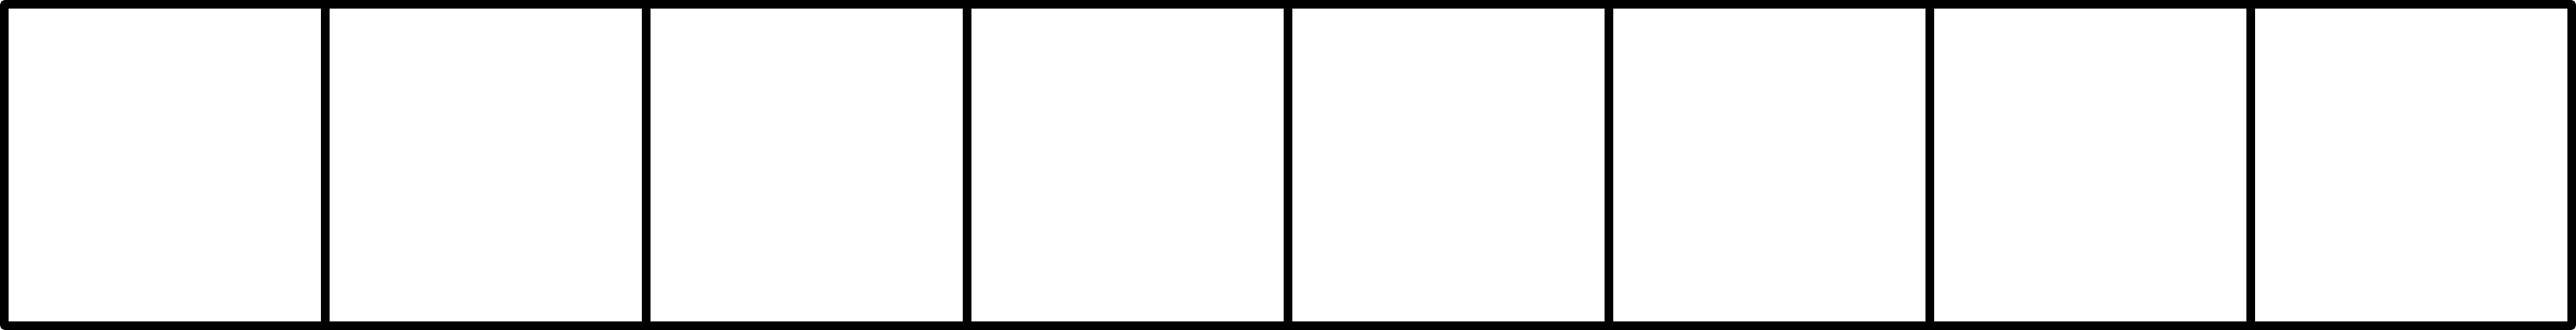
\includegraphics[width=.8\textwidth]{amortizedgfx/push_big_000.png}
  \end{center}
  }
  \only<3>{
  \begin{center}
  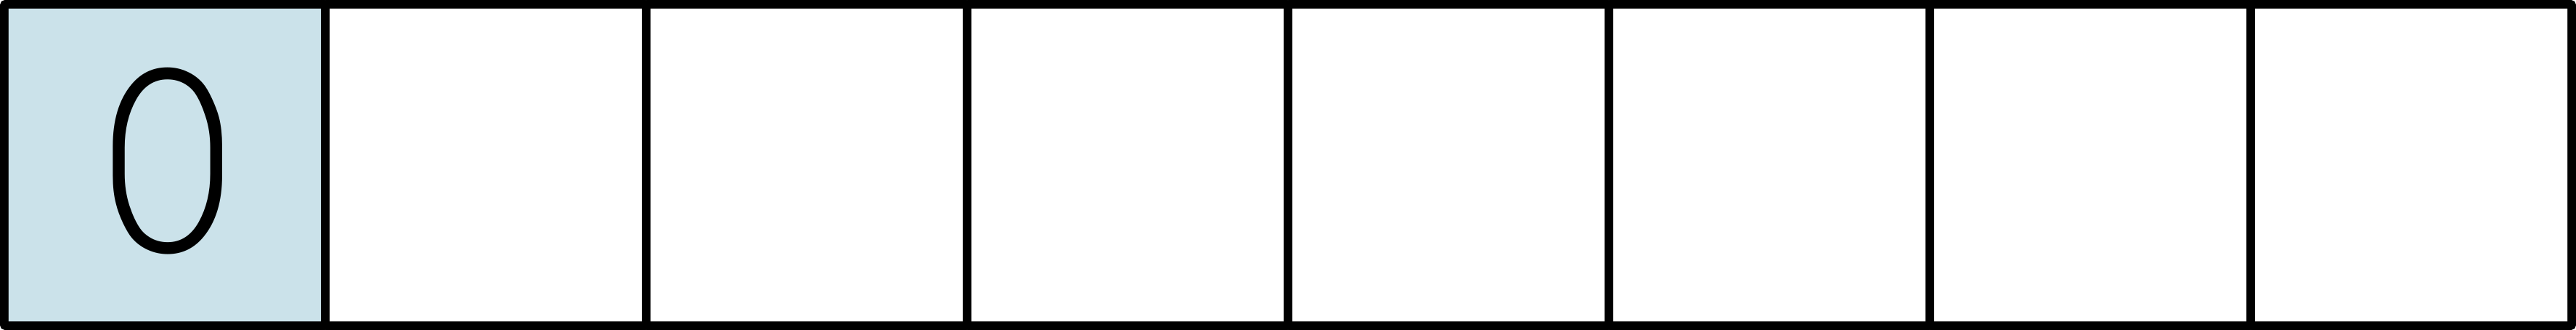
\includegraphics[width=.8\textwidth]{amortizedgfx/push_big_001.png}
  \end{center}
  }
  \only<4>{
  \begin{center}
  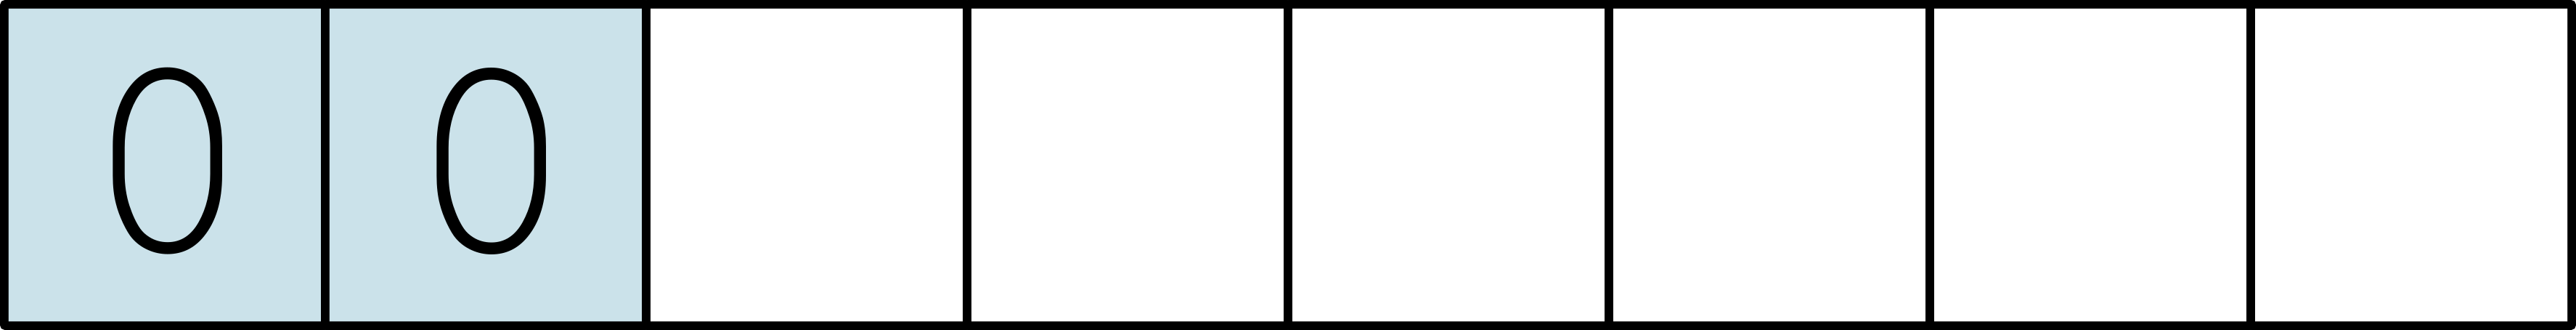
\includegraphics[width=.8\textwidth]{amortizedgfx/push_big_002.png}
  \end{center}
  }
  \only<5>{
  \begin{center}
  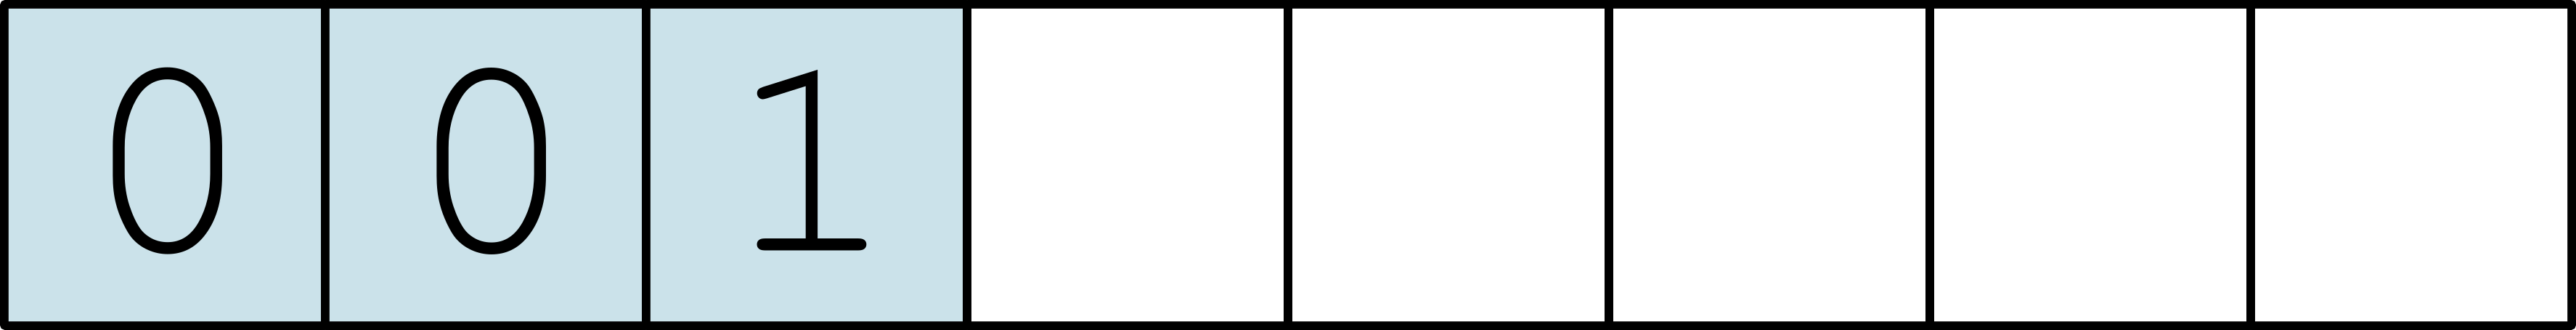
\includegraphics[width=.8\textwidth]{amortizedgfx/push_big_003.png}
  \end{center}
  }
  \only<6>{
  \begin{center}
  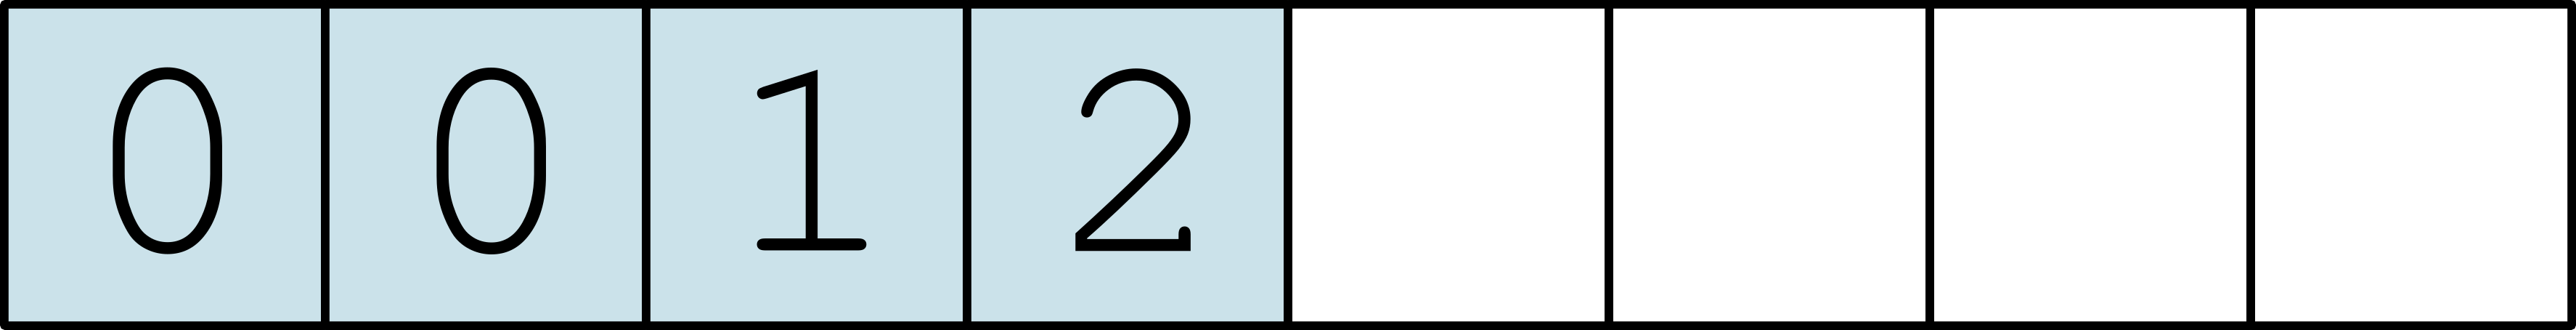
\includegraphics[width=.8\textwidth]{amortizedgfx/push_big_004.png}
  \end{center}
  }
  \only<7>{
  \begin{center}
  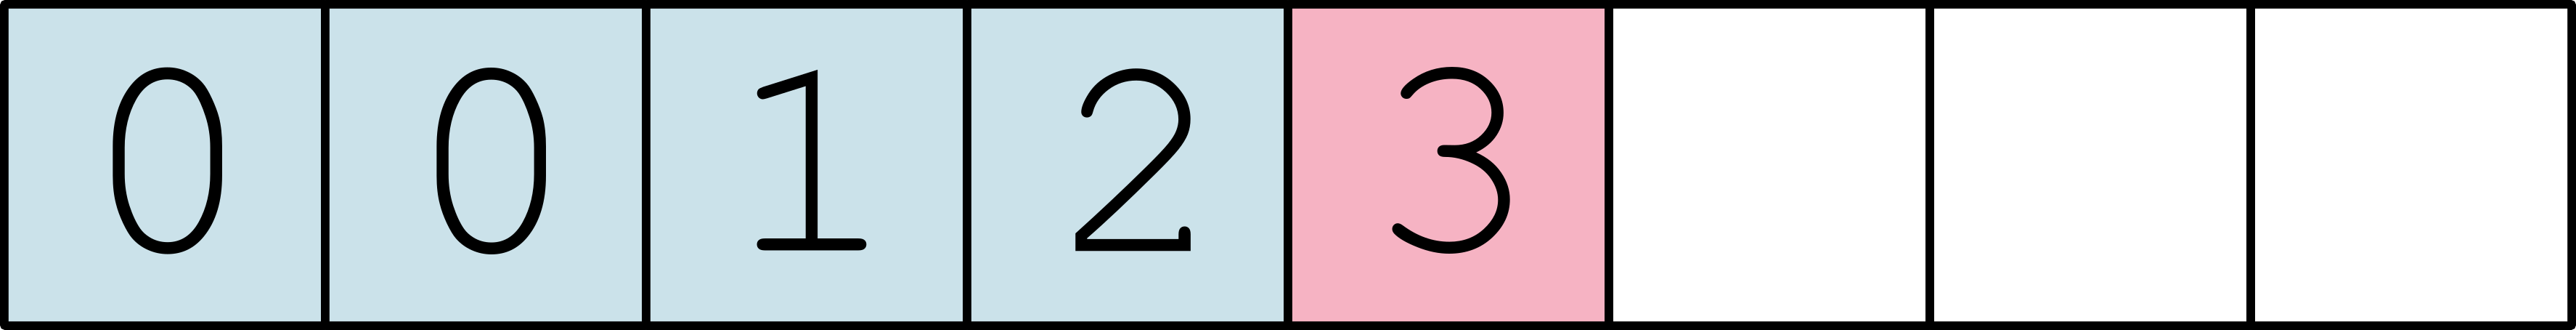
\includegraphics[width=.8\textwidth]{amortizedgfx/push_big_005.png}
  \end{center}
  }
  
  \note{
  \begin{itemize}
    \item When we want to push a third element, we have no more room available in the vector
    \item so we allocate a bigger buffer
    \item and we copy the old elements over,
    \item one by one,
    \item and for each copy
    \item we have to pay one coin.
    \item And then one more for inserting the new element.
  \end{itemize}
  }
\end{frame}

\begin{frame}
  \frametitle{Worst case complexity?}
  
  \cpause

  \begin{center}
    \huge{ $\mathcal{O}(n) $}
  \end{center}
  
  \vspace{35pt}
  
  $n$: Number of elements in the \texttt{vector}
  
  \note{
  \begin{itemize}
    \item So what is the worst case complexity of this operation?
    \item It's linear, linear in the number of elements in the vector.
  \end{itemize}
  }
\end{frame}


\begin{frame}[fragile]
  \frametitle{\texttt{push\_back} with an $\mathcal{O}(n)$ budget}
  
  \begin{tikzpicture}[remember picture,overlay]
      \node[anchor=45, shift={(0,-14ex)}] at (current page.45) {
          Budget:
          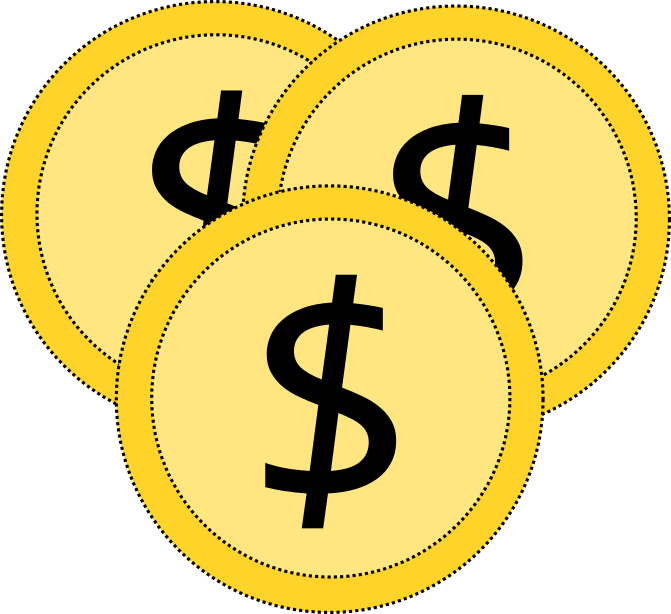
\includegraphics[keepaspectratio,
                           height=.15\textheight]{amortizedgfx/coin_03.png}
      };
  \end{tikzpicture}
  
    \begin{lstlisting}[style=cpp20]
      v.push_back(1);
    \end{lstlisting}

    \hspace{10em} Cost:
    
\includegraphics[height=.15\textheight]{amortizedgfx/coin_01.png}
    \hspace{1.5em}
    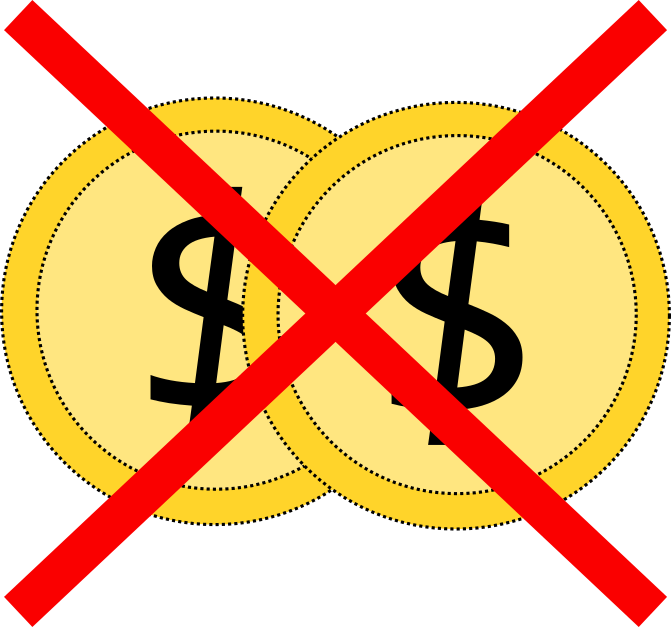
\includegraphics[height=.15\textheight]{amortizedgfx/coin_no_02.png}

    \begin{center}
      
\includegraphics[width=.5\textwidth]{amortizedgfx/push_001.png}
    \end{center}
    
  \note{
  So when pushing the first element, we have a budget of 3 coins, we need 1 coin for inserting the element and the other two we throw away.
  }
\end{frame}


\begin{frame}[fragile]
  \frametitle{\texttt{push\_back} with an $\mathcal{O}(n)$ budget}
  
    \begin{tikzpicture}[remember picture,overlay]
      \node[anchor=45, shift={(0,-14ex)}] at (current page.45) {
          Budget:
          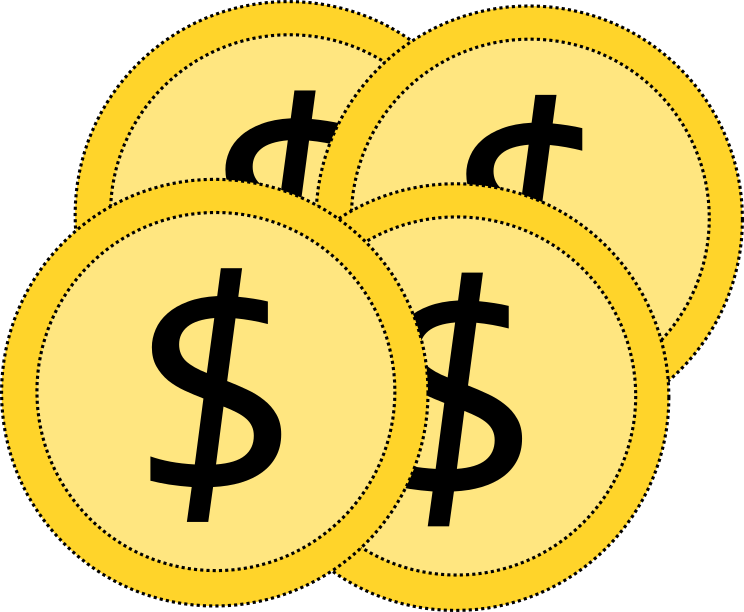
\includegraphics[keepaspectratio,
                           height=.15\textheight]{amortizedgfx/coin_04.png}
      };
  \end{tikzpicture}
  
    \begin{lstlisting}[style=cpp20]
      v.push_back(2);
    \end{lstlisting}
    
    \hspace{10em} Cost:
    
\includegraphics[height=.15\textheight]{amortizedgfx/coin_01.png}
    \hspace{1.5em}
    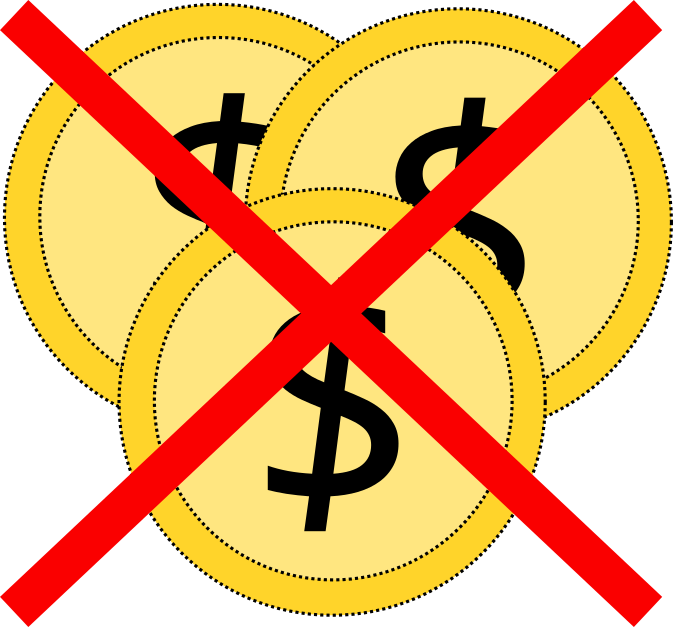
\includegraphics[height=.15\textheight]{amortizedgfx/coin_no_03.png}
    
    \begin{center}
      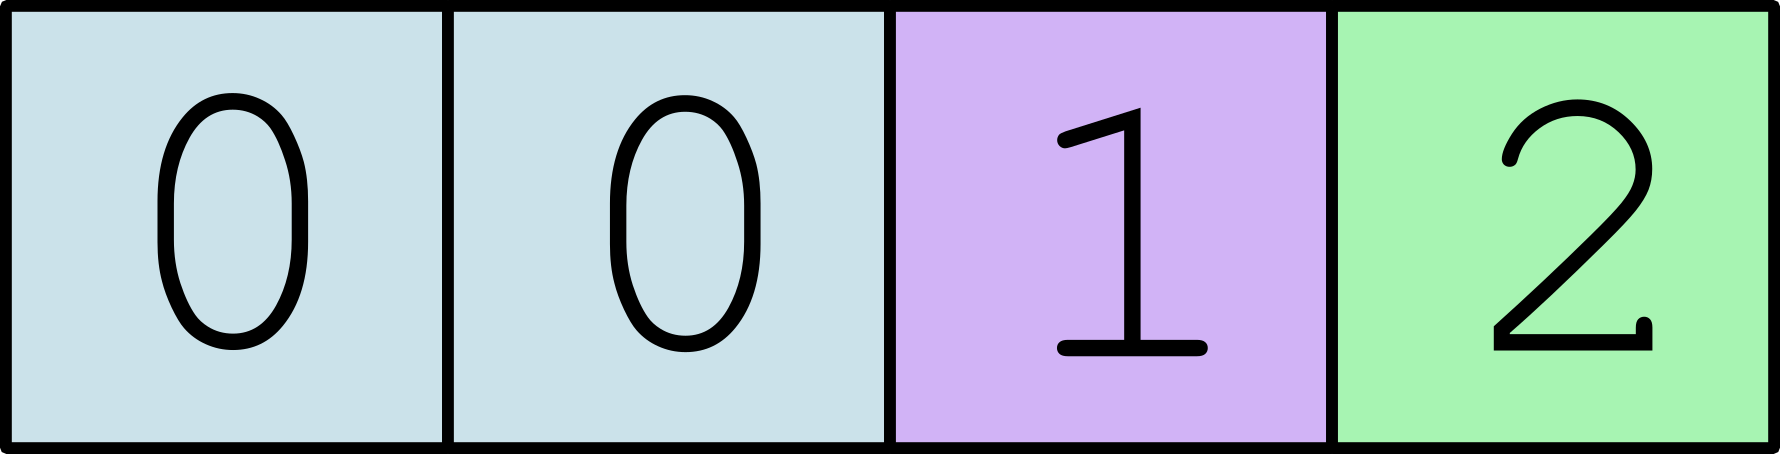
\includegraphics[width=.5\textwidth]{amortizedgfx/push_002.png}
    \end{center}
    
    \note{
    For the second element we have a budget of 4 coins, we again need 1 for the operation and throw the rest away.
    }
\end{frame}

\begin{frame}[fragile]
  \frametitle{\texttt{push\_back} with an $\mathcal{O}(n)$ budget}
  
  \begin{tikzpicture}[remember picture,overlay]
    \node[anchor=45, shift={(0,-14ex)}] at (current page.45) {
        Budget:
        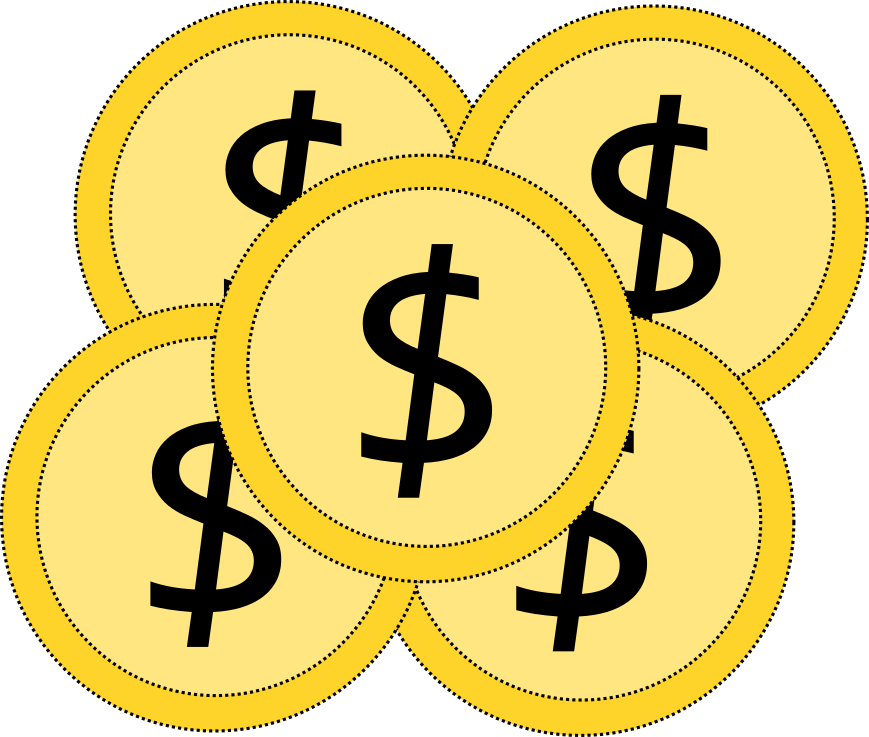
\includegraphics[keepaspectratio,
                         height=.15\textheight]{amortizedgfx/coin_05.png}
    };
  \end{tikzpicture}

    \begin{lstlisting}[style=cpp20]
      v.push_back(3);
    \end{lstlisting}

    \hspace{10em} Cost:
    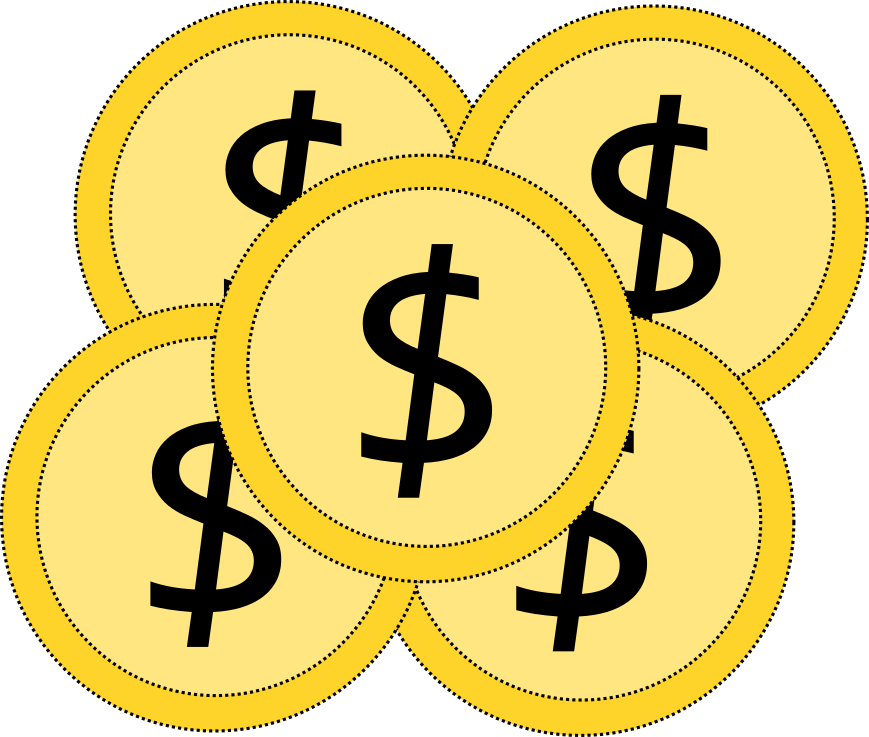
\includegraphics[height=.15\textheight]{amortizedgfx/coin_05.png}

    \begin{center}
      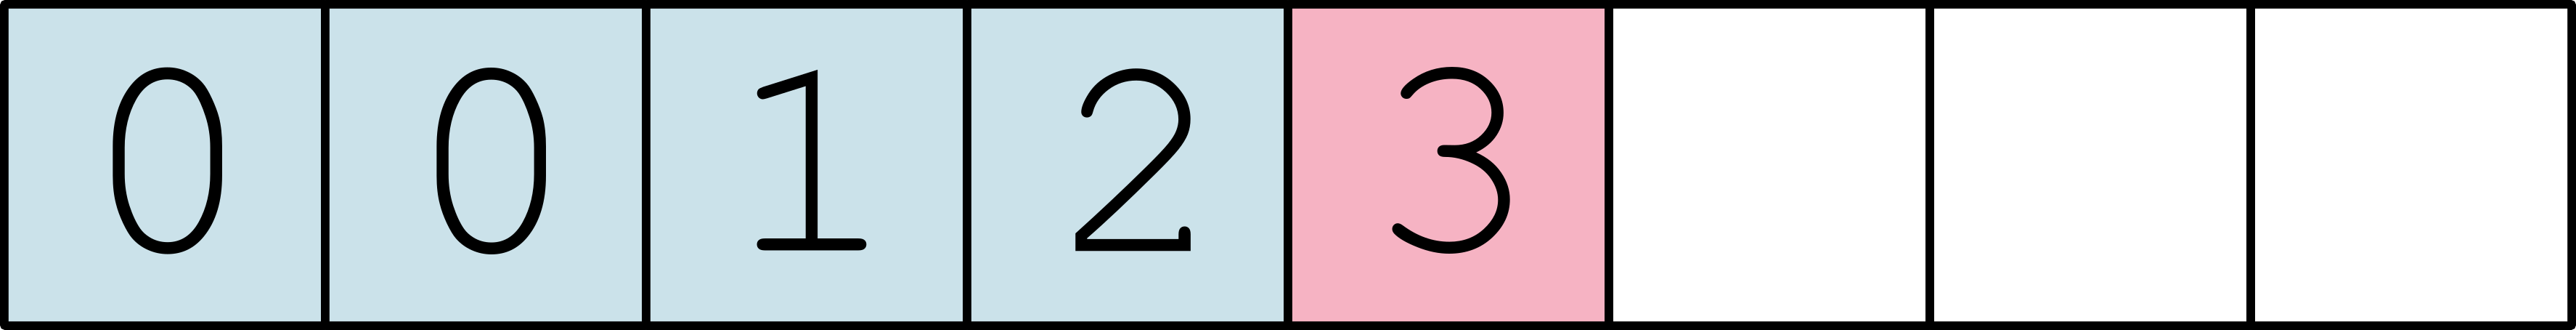
\includegraphics[width=.8\textwidth]{amortizedgfx/push_big_005.png}
    \end{center}
    
    \note{
    For the third element we have a budget of 5 coins and we need all of them to carry out the operation.
    }
\end{frame}

\begin{frame}
  \frametitle{I know what you're thinking...}
  
  That's a lot of wasted coins!
  
  \note{
  So, I know what you are thinking... We are throwing away a lot of coins!
  }
\end{frame}


\begin{frame}
  \begin{center}
    
\includegraphics[height=.8\textheight]{amortizedgfx/piggybank.png}
  \end{center}
  \tiny{
  Piggybank Image Attribution: \href{https://commons.wikimedia.org/wiki/File:Piggy_Bank_or_Savings_Flat_Icon_Vector.svg}{Videoplasty.com, CC-BY-SA 4.0 International}}
  
  \note{
  Wouldn't it be better if instead of throwing the spare coins away, we could save them somewhere and then use them to pay for subsequent operations?
  }
\end{frame}

\begin{frame}
  \frametitle{The rules of accounting}
  \begin{itemize}
  \item Each operation has a fixed budget, given by the bounding function $g$
  \item Coins that are not spent on the operation itself go into the account
  \item If an operation runs out of coins, it may take coins from the account
  \item \alert<2>{The account can not go negative. No debts!}
  \item If this works for \textit{every possible sequence of operations}, then the amortized complexity is $\mathcal{O}(g)$
  \end{itemize}
  
  \note{
  \begin{itemize}
  \item And that is exactly the idea behind accounting.
  \item One important restriction here is that our account is not allowed to go negative, I can only spend coins that I saved from earlier operations.
  \end{itemize}
  }
\end{frame}

\begin{frame}[fragile]
  \frametitle{\texttt{push\_back} with $\mathcal{O}(1)$ budget and account}
  \cpause
  
  \begin{tikzpicture}[remember picture,overlay]
    \node[anchor=45, shift={(0,-14ex)}] at (current page.45) {
        Budget:
        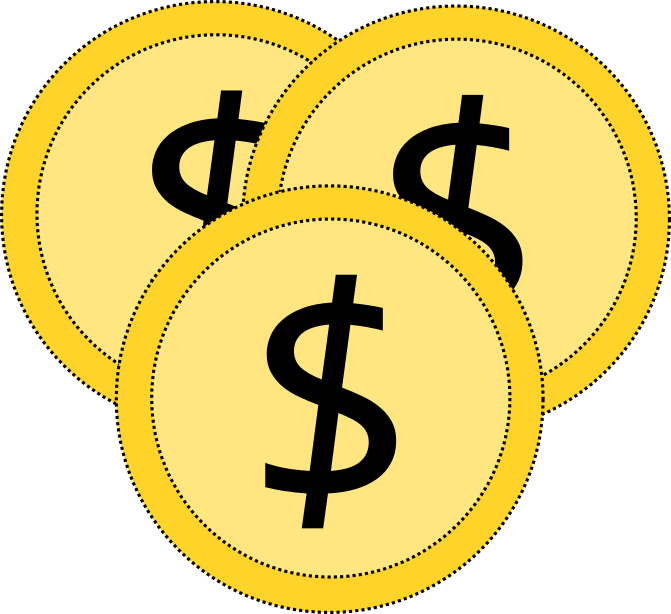
\includegraphics[keepaspectratio,
                         height=.15\textheight]{amortizedgfx/coin_03.png}
    };
  \end{tikzpicture}

  \begin{lstlisting}[style=cpp20]
    v.push_back(1);
  \end{lstlisting}
  
  \hspace{10em} Cost:
  
\includegraphics[height=.15\textheight]{amortizedgfx/coin_01.png}

  \begin{center}
    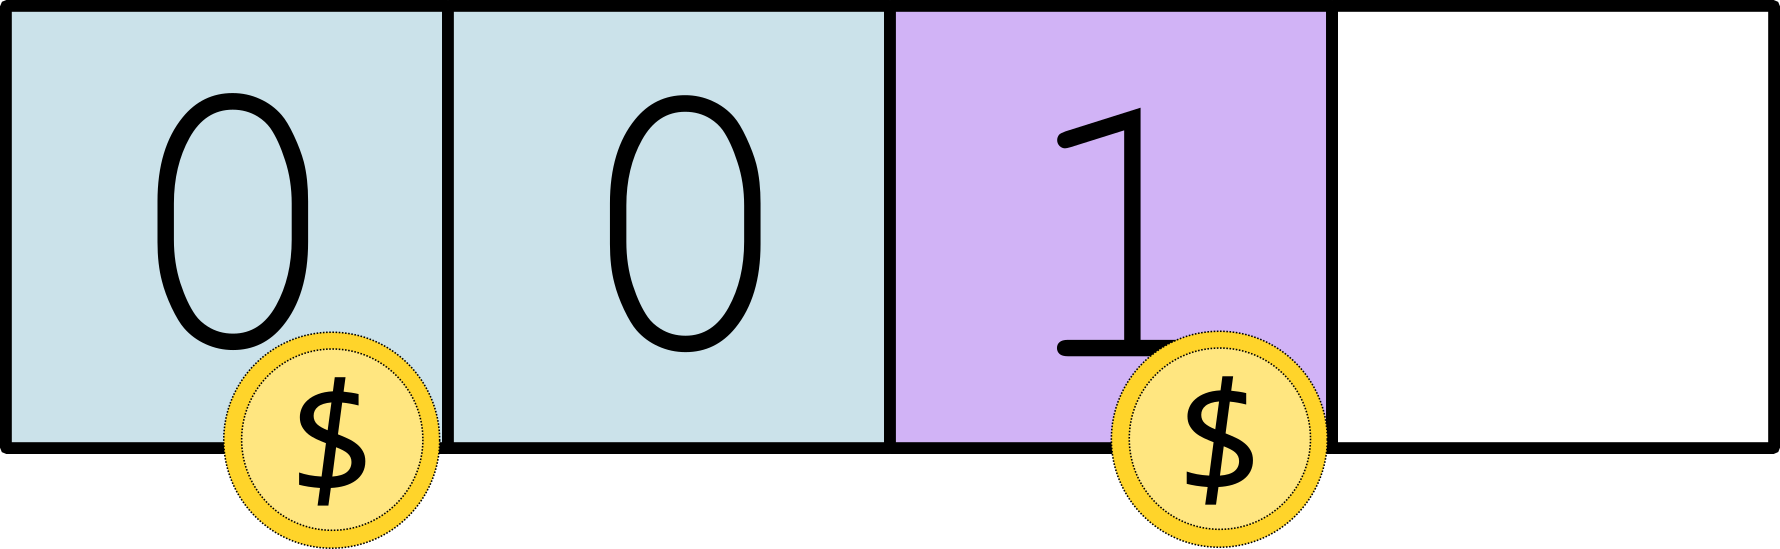
\includegraphics[width=.5\textwidth]{amortizedgfx/push_coin_001.png}
  \end{center}
  
  \note{
  \begin{itemize}
  \item Now, when following these rules, something interesting happens. We are able to execute each \texttt{push\_back} call with a constant budget of just 3 coins. Here's how it works:
  \item For the first element, I use one coin to pay for the insertion, I put the second coin on the newly inserted element and I put the third coin on one of the existing elements in the vector.
  \end{itemize}
  }
\end{frame}


\begin{frame}[fragile]
  \frametitle{\texttt{push\_back} with $\mathcal{O}(1)$ budget and account}

  \begin{tikzpicture}[remember picture,overlay]
    \node[anchor=45, shift={(0,-14ex)}] at (current page.45) {
        Budget:
        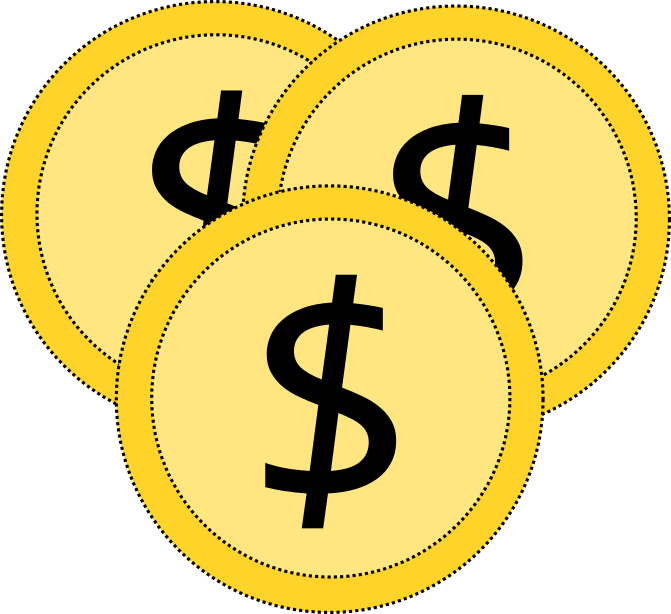
\includegraphics[keepaspectratio,
                         height=.15\textheight]{amortizedgfx/coin_03.png}
    };
  \end{tikzpicture}

  \begin{lstlisting}[style=cpp20]
    v.push_back(2);
  \end{lstlisting}
  
  \hspace{10em} Cost:
  
\includegraphics[height=.15\textheight]{amortizedgfx/coin_01.png}
  \begin{center}
    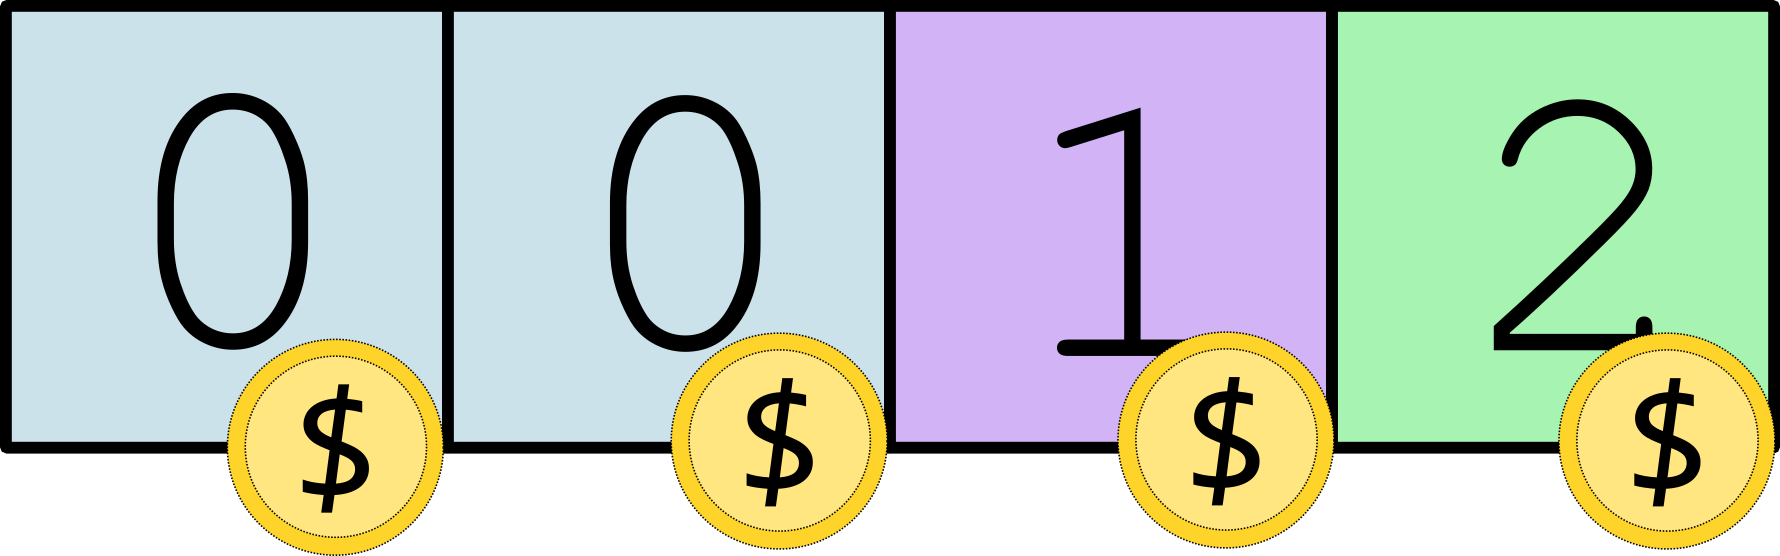
\includegraphics[width=.5\textwidth]{amortizedgfx/push_coin_002.png}
  \end{center}
  
  \note {
  I do the same with the second element.
  }
\end{frame}


\begin{frame}[fragile]
  \frametitle{\texttt{push\_back} with $\mathcal{O}(1)$ budget and account}

  \begin{tikzpicture}[remember picture,overlay]
    \node[anchor=45, shift={(0,-14ex)}] at (current page.45) {
        Budget:
        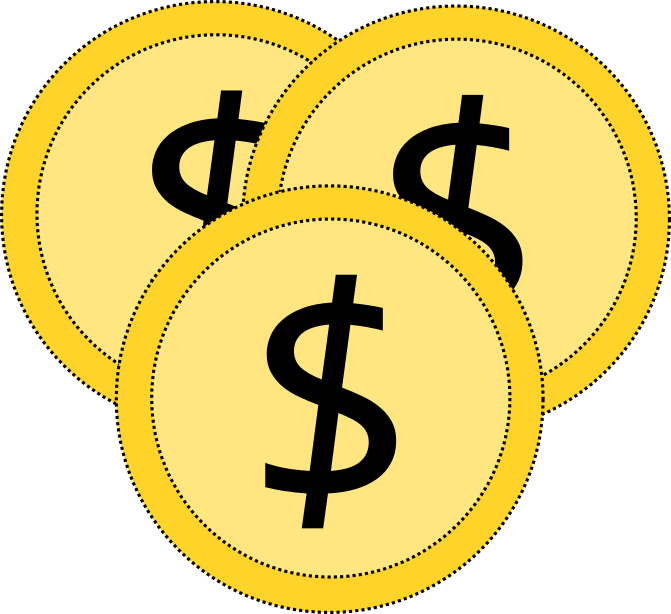
\includegraphics[keepaspectratio,
                         height=.15\textheight]{amortizedgfx/coin_03.png}
    };
  \end{tikzpicture}
  
  \begin{lstlisting}[style=cpp20]
    v.push_back(3);
  \end{lstlisting}
  
  \only<1>{
  \begin{center}
    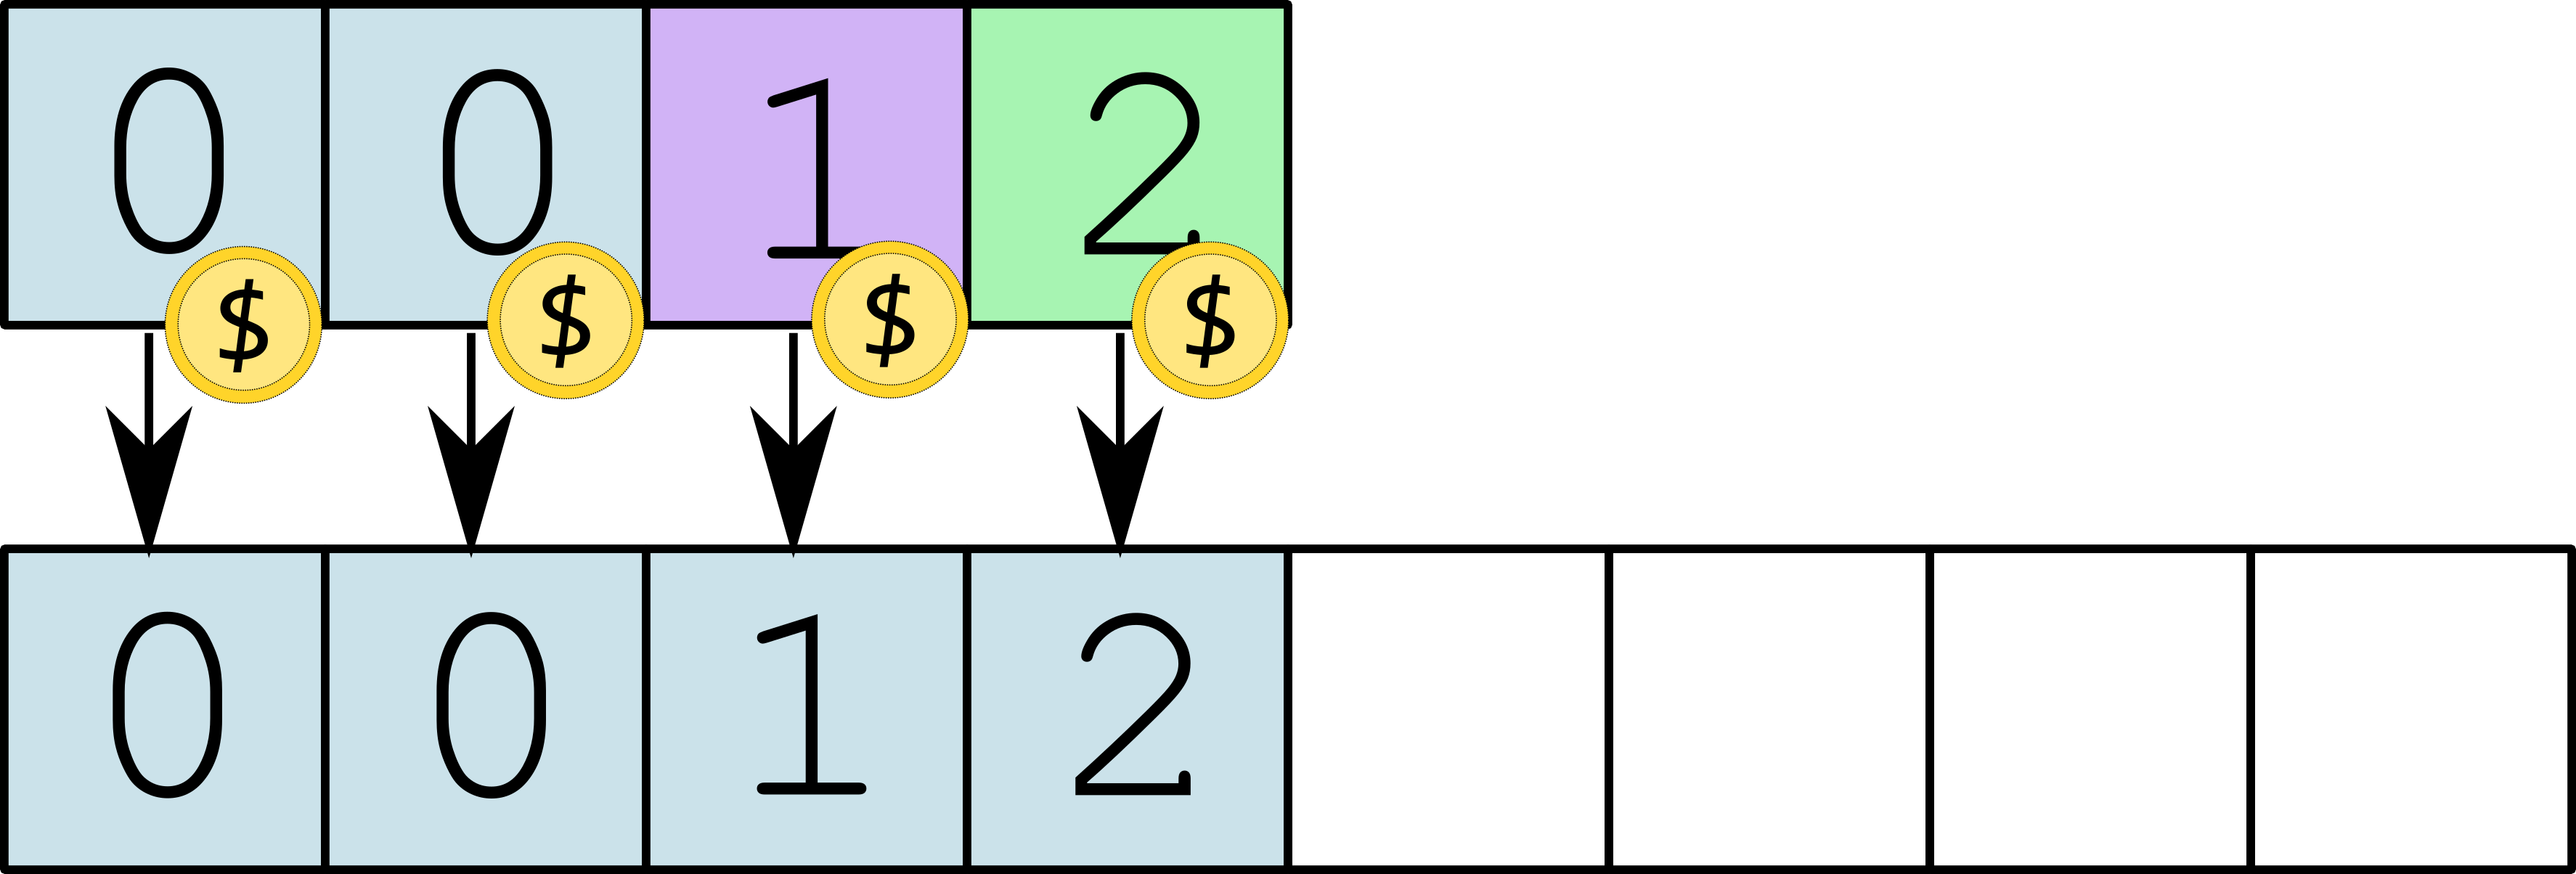
\includegraphics[width=.5\textwidth]{amortizedgfx/push_coin_copy.png}
  \end{center}
  }
  
  \only<2>{
  \hspace{10em} Cost:
  
\includegraphics[height=.15\textheight]{amortizedgfx/coin_01.png}
  \begin{center}
    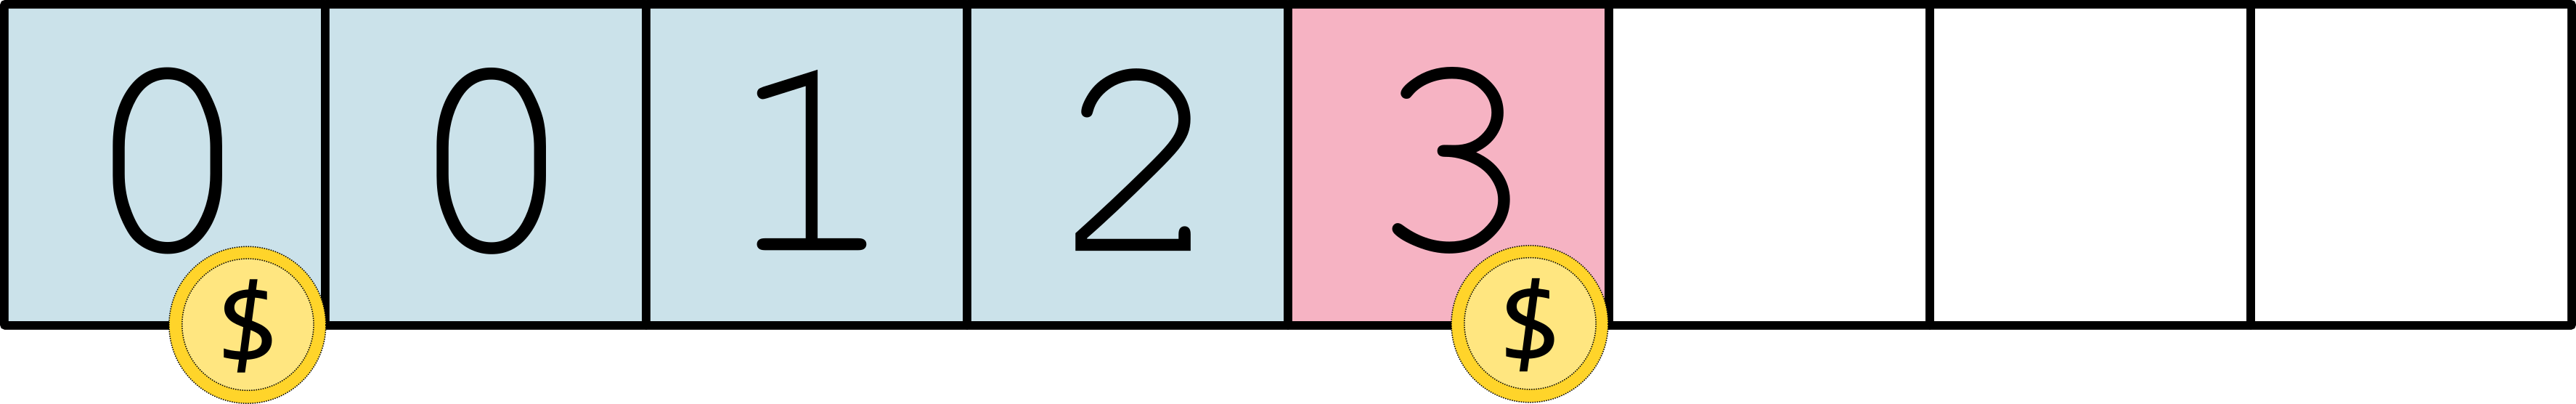
\includegraphics[width=.5\textwidth]{amortizedgfx/push_coin_003.png}
  \end{center}
  
  }
  
  \note{
  \begin{itemize}
  \item And now when inserting the third element, note how all of the existing elements in the vector already have a coin attached to them. So I can use those coins to pay for copying of the elements to the new buffer...
  \item And only use my three coins from the \texttt{push\_back} for the insertion of the new element.
  \end{itemize}
  }
\end{frame}


\begin{frame}
  \frametitle{Et voilà...}
  
  \begin{center}
    \huge{Amortized $\mathcal{O}(1)$ complexity!}
  \end{center}
  
  \note{
  And that is how amortized analysis works.
  }
\end{frame}

\begin{frame}
  \begin{center}
    
\includegraphics[height=.8\textheight]{amortizedgfx/emo_party.png}
  \end{center}
  
  \note{
  Hurray!
  }
\end{frame}

\begin{frame}
  \frametitle{Let's do another!}
  
  \cpause
  
  \begin{center}
    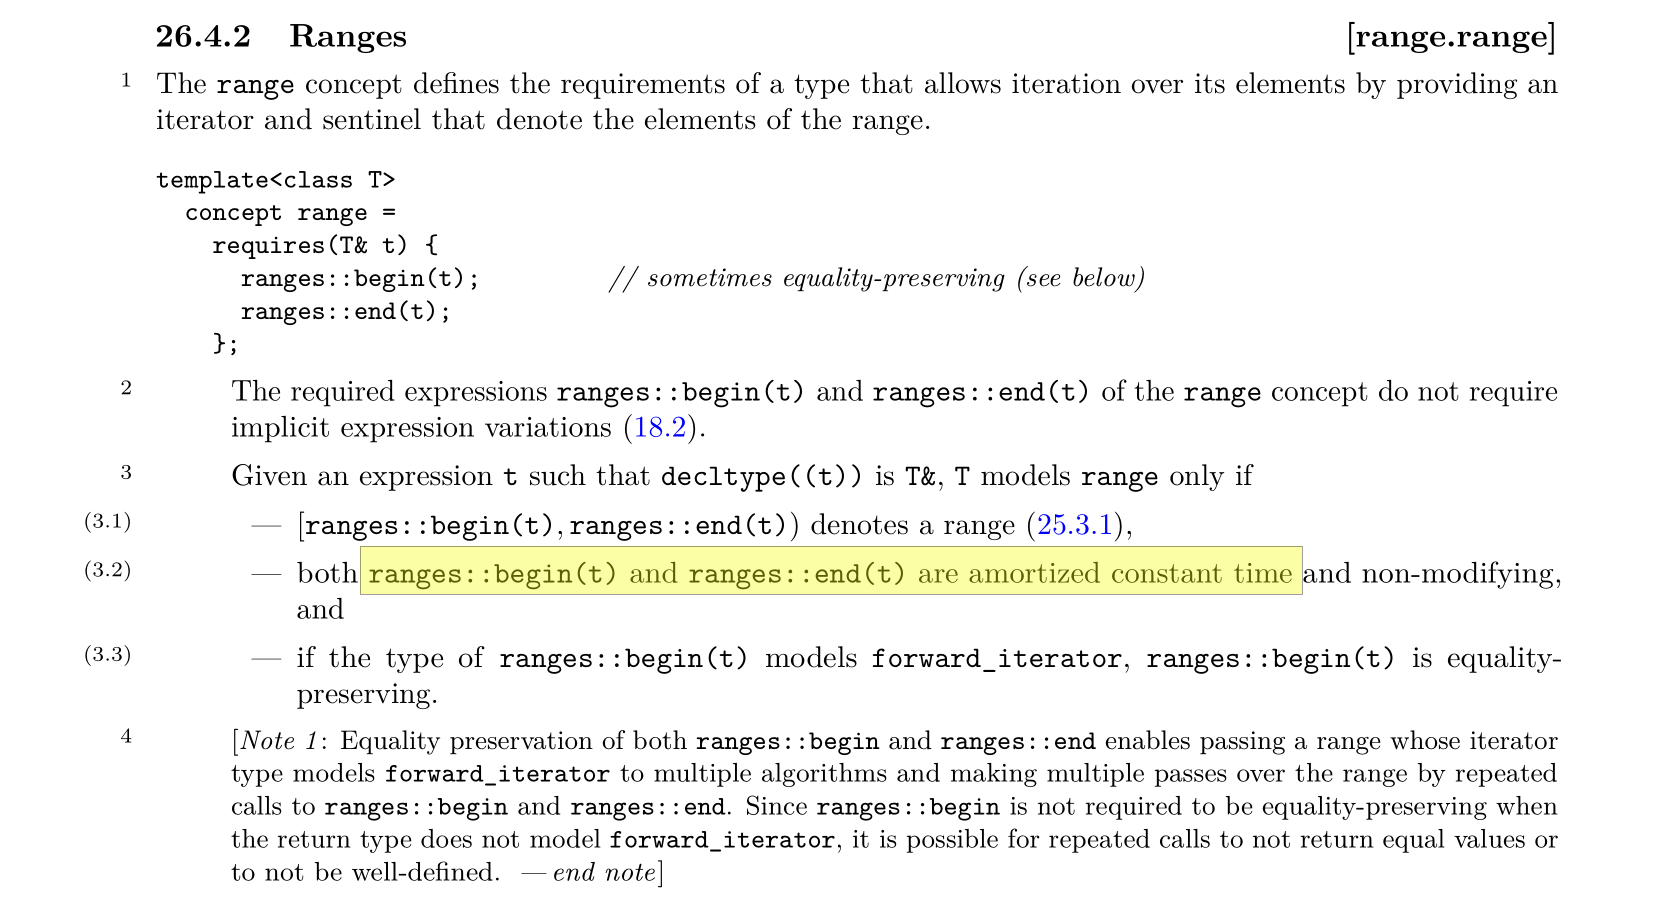
\includegraphics[height=.8\textheight]{amortizedgfx/range_range.png}
  \end{center}
  
  \note{
  \begin{itemize}
  \item We still have some time, so let's do another.
  \item The standard states that the begin() operation on a range has amortized constant complexity. How does that work?
  \end{itemize}
  }
\end{frame}


\begin{frame}[fragile]
  \frametitle{Ranges filter view}
  
  \begin{lstlisting}[style=cpp20]
    std::vector<int> v(1 << 20, 0);
    v.back() = 42;  (*@ \cpause @*)
    
    auto is_non_zero = [](int i) { return i != 0; };
    auto rng_non_zero =
      v | std::ranges::views::filter(is_non_zero);  (*@ \cpause @*)
    
    auto it1 = rng_non_zero.begin();  // O(n)
  \end{lstlisting}

  \note{
  \begin{itemize}
  \item Let's say I have a vector with a lot of zeroes and one element that I'm interested in
  \item and I want to use a filter view to get to that element.
  \item Calling \texttt{begin()} on the filter obviously has linear worst case complexity, as I need to iterate through all the zeroes that I want to filter out.
  \end{itemize}
  }
\end{frame}


\begin{frame}[fragile]
  \frametitle{Memoization!}
  
  \pause
  
  \begin{lstlisting}[style=cpp20]
    auto rng_non_zero = ...;
    
    auto it1 = rng_non_zero.begin();  // O(n)  (*@ \cpause @*)
    
    auto it2 = rng_non_zero.begin();  // O(1) (cached)
  \end{lstlisting}
  
  \note{
  \begin{itemize}
  \item But the filter also provides memoization.
  \item That means that the first call to \texttt{begin()} caches its result...
  \item and then all subsequent calls to are able to just return the cached result in constant time.
  \end{itemize}
  }
\end{frame}


\begin{frame}[fragile]
  \frametitle{Ranges find with $\mathcal{O}(1)$ budget and account}
  
  \begin{lstlisting}[style=cpp20]
  auto it1 = rng_non_zero.begin();
  \end{lstlisting}
  
  \begin{center}
    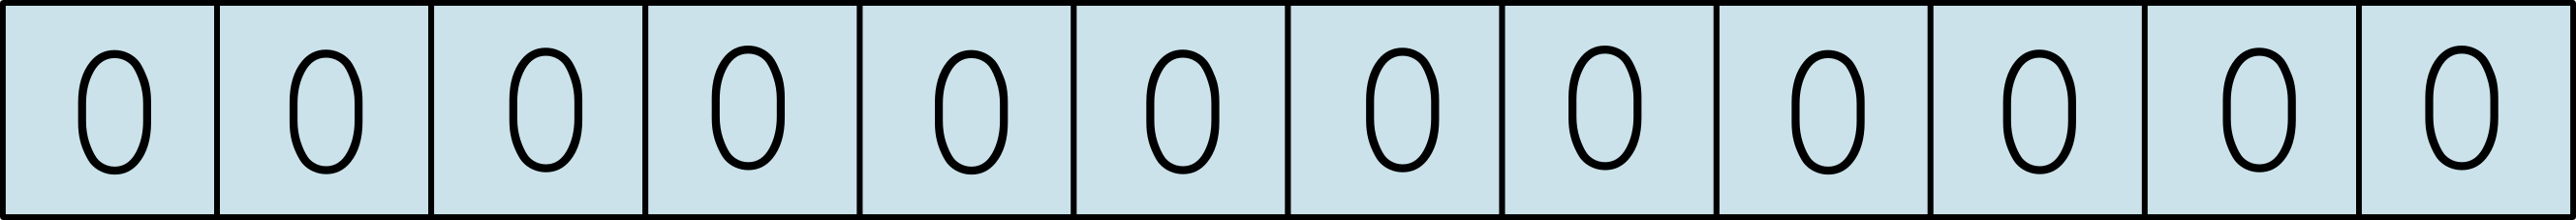
\includegraphics[height=.2\textheight]{amortizedgfx/long_vector.png}
  \end{center}
  
  \pause
  
  \begin{tikzpicture}[remember picture,overlay]
      \node[anchor=south, shift={(0,-4ex)}] at (current page.south) {
          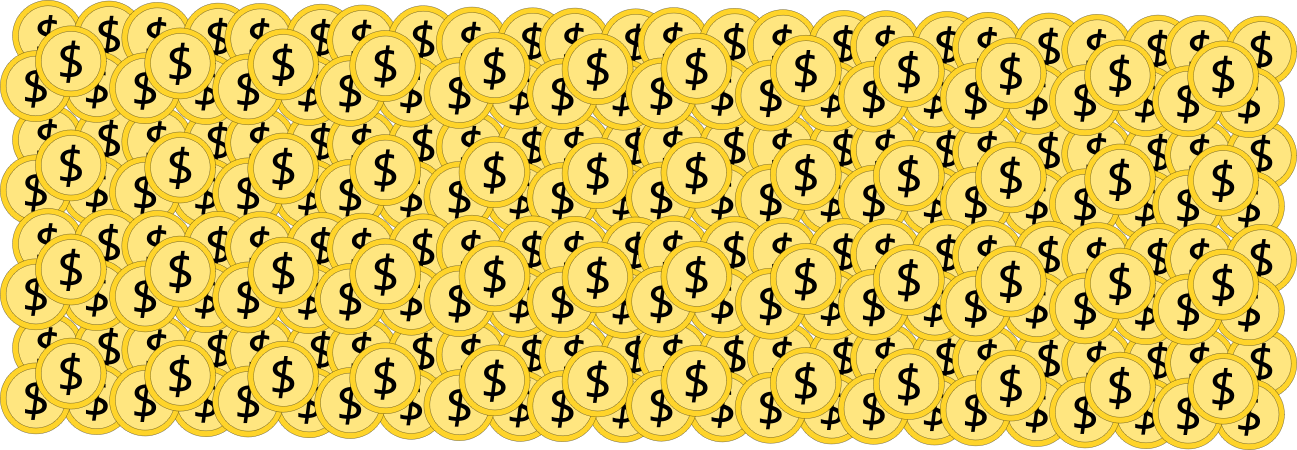
\includegraphics[keepaspectratio,
                           width=\paperwidth,
                           height=\paperheight]{amortizedgfx/coin_millions.png}
      };
  \end{tikzpicture}
  
  \note{
  \begin{itemize}
  \item So let's do the amortized analysis! We start with our vector with a million elements. When I call \texttt{begin()}...
  \item I have to pay a million coins for skipping over all the zeroes and... ... ... Yeah, this doesn't really work.
  \end{itemize}
  }
\end{frame}

\begin{frame}
  \frametitle{Let's use another method then...}
  
  \begin{itemize}
    \item Aggregate analysis
    \item \sout{Accounting method}
    \item Potential method
  \end{itemize}
  
  \note{
  But accounting was a stupid method anyway. Let's do aggregate analysis instead.
  }
\end{frame}

\fi %crop

\begin{frame}
  \frametitle{Aggregate Analysis}
  
  Let $T(n) = \sum_{i = 1}^n c_i$ be the worst case execution time for executing an arbitrary sequence of calls to \texttt{filter\_view::begin()} for a range of length $s$.
  
  $\frac{T(n)}{n}$ is the amortized cost per call.
  
  Let $c_i$ be the cost of the $i$-th call to \texttt{begin()}.
  
  Then $c_i = \left\{\begin{matrix} i=1: \mathcal{O}(s) \\ i > 1: \mathcal{O}(1) \end{matrix}\right.$.
  
  Then \alert{for $n=1$}: $T(1) = c_1 = \mathcal{O}(s)$. Thus: $\frac{T(1)}{1} = \mathcal{O}(s)$.
  
  \vspace{10pt}
  
  $\implies$ \alert{Amortized complexity is linear}.
  
  \note{
  So with aggregate analysis... it fails to be constant when there's only a single call to \texttt{begin()}.
  }
\end{frame}

\begin{frame}
  \frametitle{Potential Method}
  
  Let $c_i$ be the actual cost, and $\hat{c}_i$ be the amortized cost of the $i$th operation. Let $\Phi_i$ be the \textit{potential} of the filter view after applying the $i$th operation, and $\Phi_0 = 0$ be the initial potential.
  
  The amortized cost for the sequence of operations is

  $\sum_{i=1}^{n}\hat{c}_i = \sum_{i=1}^n( c_i ) + \Phi_n - \Phi_0$.
  
  \vspace{12pt}
  
  Assume $\forall i.\ \hat{c}_i \in \mathcal{O}(1)$. Then \alert{for $n = 1$}:
  
  $\sum_{i=1}^{1}\hat{c}_i = \hat{c}_1 \in \mathcal{O}(1)$, but $c_1 \in \mathcal{O}(s)$.
  
  Thus $\Phi_1 < 0$, which violates $\Phi_i \geq \Phi_0$ $\implies$ $\hat{c}_i$ is not a valid upper bound.
  
  \vspace{12pt}
  
  $\implies$ \alert{Amortized complexity is not $\mathcal{O}(1)$}.
  
  \note{
  And the same for the potential method.
  }
\end{frame}

\begin{frame}
  \frametitle{Runtime Complexity}
  
  \begin{center}
  \begin{itemize}
    \item $f \in \mathcal{O}(g) \iff \exists\ C > 0.\ \alert<2->{ \exists\ x_0 > 0.\ \forall\ x > x_0}: |f(x)| \le C\cdot|g(x)|$
  \end{itemize}
  \end{center}

  \vspace{12pt}
  
  \pause
  \pause

  $x$ here is the length of the input, the $n$ from the proofs before was the length of the sequence of operations!
  
  \vspace{12pt}
  
  \pause
  
  For $x$ we can ignore small numbers, for $n$ we can \textit{not}!
  
  \note{
  \begin{itemize}
  \item \alert<+>{"But wait!" - I hear you say. Complexity is only about the asymptotic case,}
  \item \alert<+>{so we don't care about a single operation.}
  \item \alert<+>{Well, no. You see, the asymptotic part here refers to the length of the input.}
  \item For the amortized analysis to be valid, the upper bound has to hold for all possible sequences of operations, even the ones that only consist of a single operation.
  \end{itemize}
  }
\end{frame}

\begin{frame}
  \begin{center}
  \huge{
  $\mathcal{O}(n)$ with memoization $\neq$ amortized $\mathcal{O}(1)$
  }
  \end{center}
  
  \note{
  So remember: These two are not the same, despite what the standard claims.
  }
\end{frame}

\begin{frame}
  \frametitle{Thanks for your attention.}

  \href{https://stackoverflow.com/users/577603/comicsansms}{\includegraphics[height=.05\textheight]{resources/so-icon.png}}
  \href{https://github.com/ComicSansMS}{\includegraphics[height=.05\textheight]{resources/github-icon.png}}
  \includegraphics[height=.05\textheight]{resources/discord-icon.png} ComicSansMS
  %\includegraphics[height=.05\textheight]{resources/discord-icon.png} ComicSansMS /
  %\href{https://twitter.com/DerGhulbus/}{\includegraphics[height=.05\textheight]{resources/twitter-icon.png} @DerGhulbus}

\end{frame}


\end{document}
